\documentclass{article}

% preamble
\def\npart{IV}
\def\nyear{2019}
\def\nterm{Lent}
\def\draft{Ongoing course, rough}
\def\nlecturer{Dr J.\ Wolf}
\def\ncourse{Connections between Model Theory and Combinatorics}

\usepackage{mathrsfs}
\usepackage{imakeidx}
\usepackage{marginnote}
\usepackage{ifthen}

\ifx \nauthor\undefined
  \def\nauthor{Bhavik Mehta}
\else
\fi

\author{Based on lectures by \nlecturer \\\small Notes taken by \nauthor}
\date{\nterm\ \nyear}
\title{Part \npart\ -- \ncourse}

\usepackage[utf8]{inputenc}
\usepackage{amsmath}
\usepackage{amsthm}
\usepackage{amssymb}
\usepackage{enumerate}
\usepackage{mathtools}
\usepackage{graphicx}
\usepackage[dvipsnames]{xcolor}
\usepackage{tikz}
\usepackage{wrapfig}
\usepackage{centernot}
\usepackage{float}
\usepackage{braket}
\usepackage[hypcap=true]{caption}
\usepackage{enumitem}
\usepackage[colorlinks=true, linkcolor=mblue]{hyperref}
\usepackage[nameinlink,noabbrev]{cleveref}
\usepackage{nameref}
\usepackage[margin=1.5in]{geometry}

% Theorems
\theoremstyle{definition}
\newtheorem*{aim}{Aim}
\newtheorem*{axiom}{Axiom}
\newtheorem*{claim}{Claim}
\newtheorem*{cor}{Corollary}
\newtheorem*{conjecture}{Conjecture}
\newtheorem*{defi}{Definition}
\newtheorem*{eg}{Example}
\newtheorem*{ex}{Exercise}
\newtheorem*{fact}{Fact}
\newtheorem*{law}{Law}
\newtheorem*{lemma}{Lemma}
\newtheorem*{notation}{Notation}
\newtheorem*{prop}{Proposition}
\newtheorem*{question}{Question}
\newtheorem*{rrule}{Rule}
\newtheorem*{thm}{Theorem}
\newtheorem*{assumption}{Assumption}

\newtheorem*{remark}{Remark}
\newtheorem*{warning}{Warning}
\newtheorem*{exercise}{Exercise}

% \newcommand{\nthmautorefname}{Theorem}

\newtheorem{nthm}{Theorem}[section]
\newtheorem{nlemma}[nthm]{Lemma}
\newtheorem{nprop}[nthm]{Proposition}
\newtheorem{ncor}[nthm]{Corollary}
\newtheorem{ndef}[nthm]{Definition}

% Special sets
\newcommand{\C}{\mathbb{C}}
\newcommand{\N}{\mathbb{N}}
\newcommand{\Q}{\mathbb{Q}}
\newcommand{\R}{\mathbb{R}}
\newcommand{\Z}{\mathbb{Z}}

\newcommand{\abs}[1]{\left\lvert #1\right\rvert}
\newcommand{\norm}[1]{\left\lVert #1\right\rVert}
\renewcommand{\vec}[1]{\boldsymbol{\mathbf{#1}}}

\let\Im\relax
\let\Re\relax

\DeclareMathOperator{\Im}{Im}
\DeclareMathOperator{\Re}{Re}
\DeclareMathOperator{\id}{id}

\definecolor{mblue}{rgb}{0., 0.05, 0.6}

\usetikzlibrary{fadings}
\swapnumbers
\reversemarginpar
\fancyfoot[R]{}

\makeindex[intoc]

\let\oldmodels\models
\let\models\vDash
\let\nModels\nvDash

\newcommand{\named}[1]{\textbf{#1}\index{#1}}
\newcommand{\bonusnamed}[1]{\textbf{#1}\index{#1@*#1}}
\newcommand{\cross}{\mathbin{\text{\rotatebox[origin=c]{-90}{$\mathrlap{\ltimes}{\rtimes}$}}}}
\DeclareMathOperator{\tp}{tp}
\DeclareMathOperator{\st}{st}
\DeclareMathOperator{\Stab}{Stab}
\DeclareMathOperator{\Sym}{Sym}
\DeclareMathOperator{\acl}{acl}
\DeclarePairedDelimiter\ceil{\lceil}{\rceil}
\DeclarePairedDelimiter\floor{\lfloor}{\rfloor}

% \setcounter{section}{-1}
\tikzset{gaplabel/.style={fill=white, rectangle, inner sep=1mm}, dot/.style={fill=black, inner sep=1pt, circle}}

% and here we go!
\begin{document}
\maketitle

\tableofcontents

\clearpage

\section{Introduction to Stability}
\subsection{History}
Shelah was interested in $I_T(\kappa)$, the number of models of $T$ of size $\kappa$ up to isomorphism.
Morley showed:
\begin{thm}
  Let $T$ be a countable theory.
  If $I_T(\kappa) = 1$ for some uncountable $\kappa$, then $I_T(\kappa)=1$ for all uncountable $\kappa$.
\end{thm}
\begin{eg}\leavevmode
  \begin{itemize}
    \item theory of vector spaces over a fixed field
    \item algebraically closed fields
  \end{itemize}
\end{eg}
\subsection{The order property}
\begin{defi}
  Let $T$ be a theory with $\mathcal{M} \models T$ and $k \geq 1$ an integer.
  Then a formula $\varphi(x,y)$ is said to have the $k$-\named{order property} if there are sequences $(a_i)_{i=1}^k$, $(b_i)_{i=1}^k$ such that $\mathcal{M} \models \varphi(a_i, b_j)$ iff $i \leq j$.
  A formula $\varphi(x,y)$ is said to be $k$-\named{stable} if it does not have the $k$-order property.
\end{defi}
\begin{eg}\leavevmode
  \begin{itemize}
    \item Take the theory of graphs, $G = \langle V, E \rangle$. The formula $E(x,y)$ is $k$-stable if $G$ does not contain a \named{halfgraph} of height $k$ as an \emph{induced bipartite subgraph} (i.e.\ we don't care about the edges between the $a_i$, similarly for the $b_j$).
      \begin{center}
        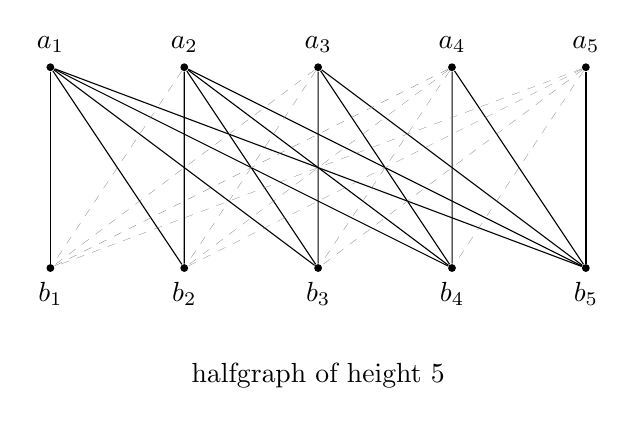
\begin{tikzpicture}[scale=1.7]
          \pgfmathsetmacro{\height}{5}
          \foreach \x in {1,...,\height} {
            \node [dot, label=below:$b_\x$] (\x1) at (\x,0) {};
          }
          \foreach \x in {1,...,\height} {
            \node [dot, label=above:$a_\x$] (\x0) at (\x,1.5) {};
            \foreach \y in {1,...,\height} {
              \ifthenelse{\x>\y}{
                \draw [dashed, ultra thin, gray] (\x0) -- (\y1);
              }
              {
                \draw (\x0) -- (\y1);
              }
            }
          }
          \node at (\height*0.5+0.5, -0.8) {halfgraph of height \height};
        \end{tikzpicture}
      \end{center}

    \item Theory of abelian groups, $\langle G, +, -, 0, A \rangle$ where $A$ is a unary predicate associated with a subset of $G$, then the formula $\varphi(x,y) = \text{`}x+y\in A\text{'} = A(+(x,y))$ is $k$-stable if $G$ does not contain
      $(a_i)_{i=1}^k, (b_j)^k_{j=1}$ such that $a_i + b_j \in A$ iff $i \leq j$.
      In this case, we say the subset $A$ is $k$-stable.
  \end{itemize}
\end{eg}
\begin{lemma}
  Let $G$ be an abelian group. If $H \leq G$, then $H$ is $2$-stable.
\end{lemma}
\begin{proof}
  Suppose $a_1, a_2, b_1, b_2$ such that $a_i + b_j \in H$ for $1 \leq i \leq j \leq 2$. Then
  \begin{equation*}
    \underbrace{(a_1 + b_1)}_{\in H} - \underbrace{(a_1 + b_2)}_{\in H} + \underbrace{(a_2 + b_2)}_{\in H} = a_2 + b_1
  \end{equation*}
  so $a_2 + b_1 \in H$.
\end{proof}
\begin{lemma}
  Let $G$ be an abelian group, $H \leq G$ and $U$ a union of $k$ cosets of $H$.  Then $U$ is $(k+1)$-stable.
\end{lemma}
\begin{proof}
  Suppose we had $a_1, \dotsc, a_{k+1}, b_1, \dotsc, b_{k+1} \in G$ witnessing the $(k+1)$-order property.
  Then by pigeonhole $\exists 1 \leq i < j \leq k+1$ such that $a_i + b_i, a_i + b_j$ lie in the same coset of $H$, whence
  $b_i - b_j \in H$ so
  \begin{align*}
    a_j + b_i = (a_j + b_j) + \underbrace{(b_i - b_j)}_{\in H} \in U.
  \end{align*}
\end{proof}
\begin{ex}
  Let $A \subseteq G$ be a Sidon set, i.e.\ it contains no non-trivial solutions to $x+y = z+w$. Show that $A$ is 3-stable.
  Are all 3-stable sets Sidon?
\end{ex}
\begin{ex}
  Show that if $A \subseteq G$ is $k$-stable, then so is $A+g$ for any $g \in G$. Moreover, $A^c$ is $(k+1)$-stable.
\end{ex}
\begin{lemma}
  Suppose $A_0, A_1 \subseteq G$ are $l$-stable and $k$-stable, respectively.
  Then $A_0 \cup A_1$ is $h(k,l)$-stable, where $h(k,l) = (k+l)2^{k+l}$.
\end{lemma}
\begin{proof}
  Suppose not. Then $\exists a_1, \dotsc, a_{h(k,l)}, b_1, \dotsc, b_{h(k,l)}$ such that $a_i + b_j \in A_0 \cup A_1$ iff $i \leq j$.

  \begin{center}
    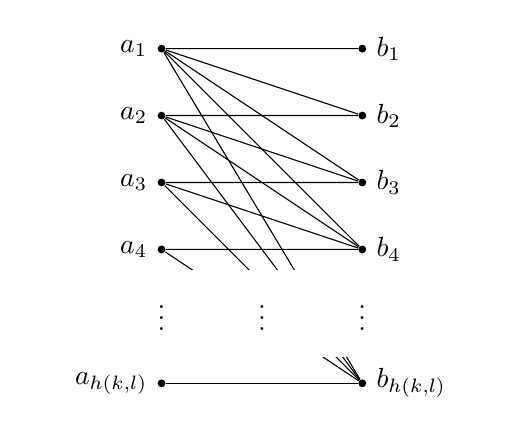
\begin{tikzpicture}[scale=1.7]
      \node [dot, label=left:$a_{h(k,l)}$] (60) at (0,1) {};
      \node [dot, label=right:$b_{h(k,l)}$] (61) at (1.5,1) {};
      \draw (60) -- (61);
      \pgfmathsetmacro{\height}{4}
        \foreach \x in {1,...,\height} {
          \node [dot, label=right:$b_\x$] (\x1) at (1.5,\height-\x/2) {};
        }
        \foreach \x in {1,...,\height} {
          \node [dot, label=left:$a_\x$] (\x0) at (0,\height-\x/2) {};
          \foreach \y in {\x,...,\height} {
            \draw (\x0) -- (\y1);
          }
          \draw (\x0) -- (61);
        }
        \draw [fill=white, draw=none] (-1,1.2) rectangle (2.5,1.85);
        \node at (0,1.55) {$\vdots$};
        \node at (0.75,1.55) {$\vdots$};
        \node at (1.5,1.55) {$\vdots$};
    \end{tikzpicture}
  \end{center}

  Since $a_1 + b_j \in A_0 \cup A_1$ for every $1 \leq j \leq h(k,l)$, there must exist $i_1 \in \{0,1\}$ and $D_1 = \{j \mid a_1 + b_j \in A_{i_1}\}$ with $|D_1| \leq h(k,l)/2$. Label $D_1$ as $j_1 < j_2 < \dotsb < j_{|D_1|}$ and define new sequences
  \begin{align*}
    a_1', \dotsc, a_{|D_1|}' &= a_1, a_{j_2}, \dotsc, a_{j_{|D_1|}} \\
    b_1', \dotsc, b_{|D_1|}' &= b_{j_1}, b_{j_2}, \dotsc, b_{j_{|D_1|}}.
  \end{align*}
  By pigeonhole, $\exists i_2 \in \{0,1\}$ and $D_2 = \{j \mid a_2' + b_j' \in A_{i_2}\}$.
  Label $D_2$ as $s_1 < s_2 < \dotsb < s_{|D_2|}$ and define new sequences
  \begin{align*}
    a_1^2 , \dotsc, a_{|D_2|}^2 &= a_1', a_2', a_{s_3}', \dotsc, a_{s_{|D_2|}}' \\
    b_1^2 , \dotsc, b_{|D_2|}^2 &= b_{s_1}', b_{s_2}', b_{s_3}', \dotsc, b_{s_{|D_2|}}'
  \end{align*}
  After $k+1$ steps, we will have sequences
  \begin{align*}
    a_1^{k+l}, \dotsc, a_t^{k+l} \\
    b_1^{k+l}, \dotsc, b_t^{k+l}
  \end{align*}
  with $t \geq \frac{h(k,l)}{2^{k+l}} = k+l$ such that for every $1 \leq j < s \leq t$, $a_s^{k+1} + b_j^{k+l} \notin A_0 \cup A_1$ and for every $1 \leq s \leq j \leq t$, $a_s^{k+l} + b_j^{k+l} \in A_{i_s}$.

  By pigeonhole again, either $\abs{\{s \mid i_s = 0\}} \geq l$ or $\abs{\{s \mid i_s = 1\}} \geq k$ contradicting the fact that $A_0$ ($A_1$) was $l$ ($k$)-stable.
\end{proof}
The typical model theoretic way of working with this is
\begin{defi}
  A formula $\varphi(x,y)$ is said to have the \textbf{order property}\index{order property!model theoretic} (OP) if there are sequences $(a_i)_{i < \omega}$, $(b_j)_{i < \omega}$ such that $\models \varphi(a_i,b_j)$ iff $i < j$.
  A formula is \textbf{stable}\index{stable!model theoretic} if it does not have the order property.
\end{defi}
\begin{ex}
  Show that any Boolean combination of stable formulas is stable.
\end{ex}
\begin{defi}
  A theory has the \textbf{order property}\index{order property!theory} if some formula in some model of the theory has the order property.
  A theory is \textbf{stable}\index{stable!theory} if it does not have the order property.
\end{defi}
\subsection{Characterisation in terms of trees}
A tree in the set theoretic sense is simply a partial order $(P, \lhd)$ such that $\forall p \in P$, $\{q \in P \mid q \lhd p\}$ is a well-order.
\begin{notation}
  \begin{align*}
    2^{< n} &= \bigcup_{i < n} \{0,1\}^i \\
    \{0,1\}^0 &= \langle \rangle \text{, the empty string}\\
    2^i &= \{0,1\}^i
  \end{align*}
  \begin{center}
    \begin{tikzpicture}
      \def\first{2.7}
      \def\second{1.4}
      \def\third{0.4}
      \node [dot, label=above:$\langle\rangle$] (-) at (0,0) {};
      \node [dot, label=above left:$0$] (0) at (-\first,-1) {};
      \node [dot, label=above right:$1$] (1) at (\first,-1) {};
      \node [dot, label=above left:$00$] (00) at (-\first-\second,-2) {};
      \node [dot, label=above right:$01$] (01) at (-\first+\second,-2) {};
      \node [dot, label=above left:$10$] (10) at ( \first-\second,-2) {};
      \node [dot, label=above right:$11$] (11) at ( \first+\second,-2) {};
      \node [dot, label=below left:$000$] (000) at (-\first-\second-\third,-3) {};
      \node [dot, label=below right:$001$] (001) at (-\first-\second+\third,-3) {};
      \node [dot, label=below left:$010$] (010) at (-\first+\second-\third,-3) {};
      \node [dot, label=below right:$011$] (011) at (-\first+\second+\third,-3) {};
      \node [dot, label=below left:$100$] (100) at ( \first-\second-\third,-3) {};
      \node [dot, label=below right:$101$] (101) at ( \first-\second+\third,-3) {};
      \node [dot, label=below left:$110$] (110) at ( \first+\second-\third,-3) {};
      \node [dot, label=below right:$111$] (111) at ( \first+\second+\third,-3) {};
      \draw [ultra thin, gray] (1) -- (-) -- (0);
      \foreach \x in {0,1,00,01,10,11} {
        \draw [ultra thin, gray] (\x1) -- (\x) -- (\x0);
      }
    \end{tikzpicture}
  \end{center}
  The set $2^{< n}$ has a natural tree structure: $\rho \unlhd \eta$ iff $\rho = \langle \rangle$ or $\rho$ is an initial segment of $\eta$.

  If $\eta = \langle \eta_1, \dotsc, \eta_i \rangle$ , $j \in \{0,1\}$ then
  \begin{equation*}
    \eta \wedge j \coloneqq \langle \eta_1, \dotsc, \eta_i, j\rangle.
  \end{equation*}
\end{notation}
\begin{defi}
  Given a graph $\Gamma = \langle V, E \rangle$, the tree bound $d(\Gamma)$ is the least integer $d$ such that there do not exist sequences $(a_\eta)_{\eta \in 2^d}, (b_\rho)_{\rho \in 2^{<d}}$ of elements of $V$ with the property that for each $\eta \in 2^d, \rho \in 2^{< d}$, if $\rho \lhd \eta$, then $a_\eta b_\rho \in E$ iff $\rho \wedge 1 \unlhd \eta$.
\end{defi}
\begin{eg}
  A graph has tree bound $2$ if it does not contain the following:
  \begin{center}
    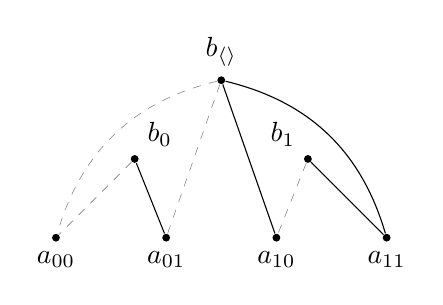
\begin{tikzpicture}
      \def\first{1.4}
      \def\second{0.7}
      \node [dot, label=above:$b_{\langle\rangle}$] (-) at (0,0) {};
      \node [dot, label=above right:$b_0$] (0) at (-\first+0.3,-1) {};
      \node [dot, label=above left:$b_1$] (1) at (\first-0.3,-1) {};
      \node [dot, label=below:$a_{00}$] (00) at (-\first-\second,-2) {};
      \node [dot, label=below:$a_{01}$] (01) at (-\first+\second,-2) {};
      \node [dot, label=below:$a_{10}$] (10) at ( \first-\second,-2) {};
      \node [dot, label=below:$a_{11}$] (11) at ( \first+\second,-2) {};
      \draw (-) -- (10);
      \draw (-) to[bend left] (11);
      \draw (0) -- (01);
      \draw (1) -- (11);
      \draw [dashed, gray, very thin] (-) to[bend right] (00);
      \draw [dashed, gray, very thin] (-) -- (01);
      \draw [dashed, gray, very thin] (0) -- (00);
      \draw [dashed, gray, very thin] (1) -- (10);
    \end{tikzpicture}
  \end{center}
\end{eg}
\begin{thm}[Shelah 1978, Hodges 1996, Alon et al 2018]
  For each $k$, $\exists d = d(k)$ such that if $\Gamma$ is a $k$-stable graph, then $d(\Gamma) \leq d$.
  (We will get $d(k) = 2^k + 1$, Hodges gives $2^{k+2} - 2$).
\end{thm}
Conversely, if $\Gamma$ contains the $2^k$-order property, then it contains a tree of height $k$.
$k=2$:
\begin{center}
  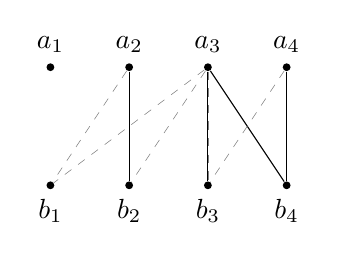
\begin{tikzpicture}
    \pgfmathsetmacro{\height}{4}
    \foreach \x in {1,...,\height} {
      \node [dot, label=below:$b_\x$] (b\x) at (\x,0) {};
    }
    \foreach \x in {1,...,\height} {
      \node [dot, label=above:$a_\x$] (a\x) at (\x,1.5) {};
    }
    \draw (a2) -- (b2);
    \draw (a3) -- (b3);
    \draw (a3) -- (b4);
    \draw (a4) -- (b4);
    \draw [dashed, gray, very thin] (a2) -- (b1);
    \draw [dashed, gray, very thin] (a3) -- (b1);
    \draw [dashed, gray, very thin] (a3) -- (b2);
    \draw [dashed, gray, very thin] (a3) -- (b3);
    \draw [dashed, gray, very thin] (a4) -- (b3);
  \end{tikzpicture}
\end{center}
More generally, a formula $\varphi$ admits a tree of height $d$ if $\exists (a_\eta)_{\eta \in 2^d}, (b_\rho)_{\rho \in 2^{< d}} \in M$ such that if $\rho \lhd \eta$, then $\models \varphi(a_\eta, b_\rho) \leftrightarrow \rho \land 1 \unlhd \eta$.

Want to show: If $G$ admits a tree of height $2^k + 1$, then $G$ has the $k$-order property.
\begin{center}
  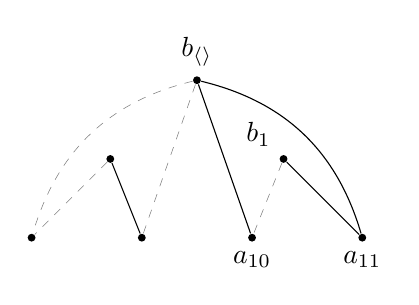
\begin{tikzpicture}
    \def\first{1.4}
    \def\second{0.7}
    \node [dot, label=above:$b_{\langle\rangle}$] (-) at (0,0) {};
    \node [dot] (0) at (-\first+0.3,-1) {};
    \node [dot, label=above left:$b_1$] (1) at (\first-0.3,-1) {};
    \node [dot] (00) at (-\first-\second,-2) {};
    \node [dot] (01) at (-\first+\second,-2) {};
    \node [dot, label=below:$a_{10}$] (10) at ( \first-\second,-2) {};
    \node [dot, label=below:$a_{11}$] (11) at ( \first+\second,-2) {};
    \draw (-) -- (10);
    \draw (-) to[bend left] (11);
    \draw (0) -- (01);
    \draw (1) -- (11);
    \draw [dashed, gray, very thin] (-) to[bend right] (00);
    \draw [dashed, gray, very thin] (-) -- (01);
    \draw [dashed, gray, very thin] (0) -- (00);
    \draw [dashed, gray, very thin] (1) -- (10);
  \end{tikzpicture}
\end{center}

% in the k=2 case, b<>, b1 is one class and a10, a11 is the other
Unfortunately, the $k=2$ case doesn't immediately generalise.
\begin{exercise}[Ramsey lemma]
  Suppose $p,q$ are positive integers and $T$ is a tree of height $p+q-1$ whose internal nodes are coloured red and blue.
  Then there is a subtree of height $p$ all of whose internal nodes are red or a subtree of height $q$ all of whose internal nodes are blue.
\end{exercise}
\begin{proof}
  Induction on $k$, where the induction statement is that the result is true, with one class a subset of leaves and the other class a subset of internal nodes.
  Assume $I(k)$, and we want $I(k+1)$.
  Given a leaf $y$, colour an internal node red if it is connected to $y$ by an edge in $G$, and blue otherwise.
  Use the Ramsey lemma on our tree, which has height $2(2^k + 1) - 1$, giving two cases
  \begin{itemize}
    \item Case 1: there is a leaf $y$ such that we get a red subtree $T'$ of height $2^k + 1$, say its root is $x$ (include the leaves too).
      Let $T''$ be the subtree of $T'$ rooted at the left child of $x$.
      Note that $T''$ has height $2^k$

      Let $X', Y'$ be the set of leaves, nodes of $T''$, respectively
      Note that no element of $Y'$ connects to $\eta$ in $G$.
      By the inductive hypothesis, we find $X_0 \subseteq X'$, $Y_0 \subseteq Y'$ that give a half graph of height $k$.

      Observe $y \in Y_0$. Let $X = X_0 \cup \{x\}$, $Y = Y_0 \cup \{y\}$.
      $y$ is connected to everything in $X_0$ but $x$ is connected to nothing in $Y_0$, giving the required halfgraph.
    \item Case 2: Suppose no leaf $y$ produces a red subtree of height $2^k + 1$.
      Say $x$ is the root of $T$, and say $T'$ is the subtree rooted at the right child of $x$, and consider only the leaves of $T'$.

      Pick a leaf of $T'$. This, by assumption, induces a blue subtree $T''$ in $T'$ of height $2^k$ in $T'$.

      By the inductive hypothesis, there are $X_0,Y_0$ which give a halfgraph of height $k$ using $X = \{x\} \cup X_0$, $Y = \{y\} \cup Y_0$ (attached to the front). \qedhere
  \end{itemize}
\end{proof}
\begin{exercise}
  Show that the theory of the random graph is unstable.
\end{exercise}
\subsection{Characterisation of stability in terms of types}
\begin{defi}
  Let $\mathscr{M} \models T$, $A \subseteq M$ a set of parameters, $\varphi(x,y)$ a formula.
  Then a (partial) $\varphi$-type over $A$ is a collection of formulas of the form $\varphi(x,a)$, $\neg \varphi(x,a)$ for some $a \in A$.
\end{defi}
\begin{defi}
  A complete $\varphi$-type over $A$ is a maximal consistent partial type over $A$ (i.e.\ $\forall a \in A$, either $\varphi(x,a)$ or $\neg \varphi(x,a)$ is in the type).
  Let $S \varphi(A)$ denote the space of complete $\varphi$-types over $A$.
\end{defi}
\begin{eg}
  $G = \langle V,E \rangle$, $A \subseteq V$, $\varphi(x,y) = E(x,y)$. Suppose $A = \{a_1,a_2,a_3,a_4\}$
  Then a possible type is $p(x) = \{E(x,a_1), E(x,a_2), \neg E(x,a_3)\}$, and the type defines the set of vertices which connect to $a_1$ and $a_2$ but not to $a_3$.
  \begin{center}
    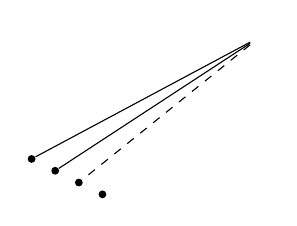
\begin{tikzpicture}
      \begin{scope}[every node/.style={inner sep=1pt, fill=black, circle}, xscale=0.3, yscale=0.15]
        \node (a4) at (0,0) {};
        \node (a3) at (-1,1) {};
        \node (a2) at (-2,2) {};
        \node (a1) at (-3,3) {};
      \end{scope}
      \node (x) at (2,2) {};
      \draw (x) -- (a1);
      \draw (x) -- (a2);
      \draw [dashed] (x) -- (a3);
    \end{tikzpicture}
  \end{center}
  $p(x)$ is not complete, but if, say, $\neg E(x,a_4)$ were added, then it is a complete $E$-type over $A$.
\end{eg}
% lecture 4
\begin{defi}
  Let $b \in M$, $A \subseteq M$. Then the type of $b$ over $A$ is the collecitno of all formulas with parameters in $A$ that are satisfied by $b$:
  \begin{equation*}
    \tp_\varphi(b/A) \coloneqq \{\varphi(x,a) \mid a \in A, \models \varphi(b,a)\}.
  \end{equation*}
\end{defi}
We have
\begin{equation*}
  S\varphi(A) \supseteq \{\tp_\varphi(b/A) \mid b \in M\}.
\end{equation*}
\begin{ex}\leavevmode
  \begin{enumerate}[label=(\roman*)]
    \item Prove the Erd\H{o}s-Makkai theorem:
      Let $A$ be an infinite set and let $\mathcal{F} \subseteq \mathcal{P}(A)$ such that $|\mathcal{F}| > |A|$. Then there are sequences $(a_i)_{i < \omega}$, $a_i \in A$, $(F_j)_{j < \omega}$, $F_j \in \mathcal{F}$ such that either
      \begin{align*}
        \text{either }a_i \in F_j &\leftrightarrow j < i \; \forall i,j \in \omega \\
        \text{or }a_i \in F_j &\leftrightarrow i < j \; \forall i,j \in \omega
      \end{align*}
    \item Deduce that if $|S\varphi(A)| > |A|$, then $\varphi(x,y)$ is unstable.
  \end{enumerate}
\end{ex}
\begin{thm}
  Let $G = (V,E)$ be an infinite graph. Suppose $\exists$ countable $A \subseteq V$ such that
  \begin{equation*}
    \abs{\{\{a \in A \mid E(a,b)\} \mid b \in V\}} > \aleph_0.
  \end{equation*}
  Then $G$ contains an infinite halfgraph.
\end{thm}
\begin{proof}
  Pick an uncountable sequence $(c_i)_{i < \omega_1}$, of distinct elements of $V$, each inducing a different partition of $A$.
  By induction on $n < \omega$, we define an increasing sequence of countable sets $A_n \subseteq V$ as follows:
  \begin{itemize}[label=--]
    \item $A_0 \coloneqq A$
    \item having constructed $A_n$ for some $n \geq 0$, we choose $A_{n+1} \supseteq A_n$ such that $\forall$ finite $B \subseteq A_n$, every partition of $B$ which is induced by a vertex in $V$ is already induced by a vertex in $A_{n+1}$.
  \end{itemize}
  Remark: $A_{n+1}$ is countable, since there are countably many $B$, and we only need to add in one vertex each.
  \begin{center}
    \begin{tikzpicture}[scale=1.8]
      \draw (0,0) ellipse (3.5cm and 2.5cm);
      \draw (-0.5,0.4) ellipse (2.5cm and 1.7cm);
      \draw (-0.9,0.7) ellipse (1.2cm and 0.7cm);
      \draw (0.3,0.2) circle (0.8);
      \node [gaplabel] at (-0.9,1.4) {$A_0=A$};
      \node [gaplabel] at (-0.5,-1.3) {$A_n$};
      \node [gaplabel] at (0,-2.5) {$A_{n+1}$};
      \node [gaplabel] at (0.5,0.98) {$B$};
      \draw [bred, shift={(0.3,0.2)}] (130:0.8) -- (-50:0.8);
    \end{tikzpicture}
  \end{center}
  Claim: $\exists i < \omega_1$ such that $\forall n < \omega$, $\forall$ finite $B \subseteq A_n$, we can find two elements $v = v_{n,B}$ and $w = w_{n,B}$ in $A_{n+1} \setminus \{c_i\}$ such that $v$ and $w$ induce the same partition on $B$ but $E(c_i,v)$ and $\neg E(c_i,w)$.

  For now, assume this claim, and construct the halfgraph.
  Fix $c_* = c_i$ for $i < \omega$ in the claim. We will construct three vertex classes, and use a Ramsey argument to give the halfgraph. Construct sequences $(a_n)_{n < \omega}, (b_n)_{n < \omega}, (c_n)_{n < \omega}$ with $a_n, b_n, c_n \in A_{2n+2}$.
  Having completed step $n-1$, let
  \begin{equation*}
    B_n = \bigcup_{m < n} \{a_m, b_m, c_m\}.
  \end{equation*}
  Note that $B_n \subseteq A_{2(n-1)+2} = A_{2n}$.
  By choice of $c_*$, $\exists a_n, b_n \in A_{2n+1} \setminus \{c_*\}$ such that $E(c_*, a_n), \neg E(c_*, b_n)$ and $a_n$ and $b_n$ induce the same partition on $B_n$.

  To complete step $n$, choose $c_n \in A_{2n+2}$ such that it induces the same partition of $B_n \cup \{a_n, b_n\}$ as $c^*$. (Note $c^*$ and $c_n$ induce the same partition on $B_n$, but this doesn't have to be the same partition that $a_n$ and $b_n$ induce on $B_n$).

  Observe:
  \begin{itemize}
    \item if $m > n$, then $a_m$ and $b_m$ relate to $c_n$ in the same way: $E(a_m ,c_n) \leftrightarrow E(b_m, c_n).$ % yellow
    \item if $m \leq n$, $c_*$ and $c_n$ relate to $a_m$ and $b_m$ in the same way, and $\forall m$, $E(a_m, c^*)$ and $\neg E(b_m, c^*)$. % red
      So $E(a_m, c_n)$ and $\neg E(b_m, c_n)$ for all $m \leq n$.
  \end{itemize}

  If $ E(a_m, c_n)$ on an infinite subsequence, $E(b_m, c_n) \leftrightarrow n < m$. If not, $E(a_m, c_n) \leftrightarrow m \leq n$.

  Finally, it remains to prove the claim.
  Suppose the conclusion fails. Then $\forall i < \omega_1$, $\exists n < \omega$, $\exists$ finite $B \subseteq A_n$ such that whether or not $c_i$ connects to $v \in A_{n+1} \setminus \{c_i\}$ is entirely determined by the partition of $B$ induced by $v$.

  Replacing $(c_i)_{i<\omega_1}$ by a subsequence, may assume that $n$ is constant and $B$ is constant. Fix $n,B$.
  By construction, since $B$ is finite, $\exists$ finite $C \subseteq A_{n+1}$ such that every partition of $B$ is already induced by an element of $C$.
  \begin{enumerate}[label=(\arabic*)]
    \item By passing to a subsequence, may assume that all $(c_i)_{i < \omega_1}$ induce the same partition on $C$.
    \item Any two $c_i$s induce distinct partitions on $A$, so $\exists a_* \in A$ such that $E(c_i, a_*)$ but $\neg E(c_j, a_*)$.
    \item By choice of $C$, there is $a_{**} \in C$ such that $a_*$ and $a_{**}$ induce the same partition on $B$.
    \item But $B$ is such that whether or not $v \in A_{n+1} \setminus \{c_i\}$ is connected to $c_i$ is entirely determined by the partition it induces on $B$.
  \end{enumerate}

\end{proof}
\section{Applications of stability}
\subsection{Stable Ramsey/\texorpdfstring{Erd\H{o}s}{Erdos}-Hajnal}
\begin{defi}
  Let $A \subseteq 2^{<n}$ be closed under initial segments (CUIS) and let $G$ be a graph on $n$ vertices.
  We say $G$ \textbf{is a type tree}\index{type tree} on $A$ if there is an indexing $V = \{a_\eta : \eta \in A\}$ such that $\forall \eta \in A$, the following holds.
  \begin{enumerate}[label=(\arabic*)]
    \item If $\eta \wedge 0$ is in $A$, then $\neg E(a_\eta, a_{\eta \wedge 0})$
    \item If $\eta \wedge 1$ is in $A$, then $E(a_\eta, a_{\eta \wedge 1})$
    \item If $\sigma,\tau \in A$ and $\eta \lhd \sigma \lhd \tau$, then
      \begin{equation*}
        E(a_\eta, a_\sigma) \leftrightarrow E(a_\eta, a_\tau)
      \end{equation*}
  \end{enumerate}
  A type tree of $A$ has height $h$ if $A \subseteq 2^{<h}$ but $A \nsubseteq 2^{<h-1}$
\end{defi}
\begin{lemma}
  Every graph on $n$ vertices is a type tree on $A$ for some $A \subseteq 2^{<n}$ (CUIS).
\end{lemma}
\begin{proof}

  Let $a_{\langle \rangle}$ be an arbitrary element of $V$.
  Let $A_0 = \{a_{\langle\rangle}\}$, $X_{\langle\rangle} = V$.
  Set $X_1 = N_G(a_{\langle \rangle})$, $X_0 = V \setminus (N_G(a_{\langle\rangle}) \cup \{a_{\langle\rangle}\})$
  Observe $X_0$ and $X_1$ partition $V \setminus A_0$.

  Suppose we've constructed $A_0, A_1, \dotsc, A_m$ for $m \geq 0$, and that for each $\eta \in A_m$, we have a partition of $X_\eta$ with the following properties:
  \begin{enumerate}
    \item $\{X_{\eta \wedge i}: \eta \in A_m, i=0,1\}$ partition $V \setminus \bigcup_{i=0}^m \{a_\eta : \eta \in A_i\}$
    \item $\forall \eta \in A_m$, $X_{\eta \wedge 1} \subseteq N_G(a_\eta)$, $X_{\eta \wedge 0} \subseteq V \setminus (\{a_\eta\} \cup N_G(a_\eta)).$
  \end{enumerate}

  Now for each $\eta \in A_m$ and $i \in \{0,1\}$ let $a_{\eta \wedge i}$ be an arbitrary element of $X_{\eta \wedge i}$ be an arbitrary element of $X_{\eta \wedge i}$. If $X_{\eta \wedge i} \neq \emptyset$. Let $A_{m+1}$ be the set of all these elements.

  For each $\sigma \in A_{m+1}$, $i \in \{0,1\}$,
  \begin{align*}
    X_{\sigma \wedge 1} = N(a_0) \cap X_0 \\
    X_{\sigma \wedge 0} = (V \setminus (\{a_0\} \cup N_G(a_d))) \cap X_\sigma
  \end{align*}
  Check that the set $A = \bigcup_{i=1} A_i$ satisfies the properties of a type tree.
\end{proof}
\begin{defi}
  Say $G=(V,E)$ contains a type tree of height $h$ if $\exists V' \subseteq V$ such that the induced graph on $V'$ is a type tree of height $h$ on $A$ for some $A \subseteq 2^{<h}$ (CUIS).

  The tree height of $G$, denoted by $h(G)$ is the largest $h$ such that $G$ contains a type tree of height $h$.
\end{defi}
\begin{defi}
  Say $G = (V,E)$ contains a full binary type tree of height $t$ if $\exists V' \subseteq V$ such that the induced graph on $V'$ is a type tree on the set $2^{<t}$.
  The tree rank of $G$, $t(G)$ is the largest full binary type tree of height $t$.
\end{defi}
Observe that $d(G) \leq k$ then $t(G) \leq k$.
Observe also that if $G$ has tree rank $t$, then $G$ contains an independent set of size $t$.

\begin{lemma}
  Let $h \geq 1$ and let $G=(V,E)$ be a finite graph of tree height $h$. Then $G$ contains a clique or an independent set of size $\geq \frac{h}{2}$.
\end{lemma}
\begin{proof}
  Since $G$ has tree height $h$, $\exists V' \subseteq V$ such that $V' = \set{a_\eta | \eta \in A}$ for some $A \subset 2^{<h}$ containing a branch $B$ of length $h$. Let $a_\tau$ be the final element of $B$.
  By assumption, $|B| = h$. If $|N(a,\tau) \cap B| \geq \frac{h}{2}$, then let $I = N(a_\tau) \cap B$, otherwise let
  \begin{equation*}
    I = (V \setminus N(a_\tau)) \cap B.
  \end{equation*}
  If $x,y \in I$, then by definition of $I$,
  \begin{align*}
    E(a_\tau, x) \leftrightarrow E(a_\tau,y).
  \end{align*}
  But by (3), in the definition of a type tree, $E(a_\tau, x) \leftrightarrow E(x,y)$.
\end{proof}
\begin{thm}[Malliaris-Shelah 2014, Malliaris-Terry 2016]
  % For all integers $k$, $\exists c = c(k)$ and $\delta = \delta(k)$ such that the following holds. Let $n \geq 2$ be an integer and let $G$ be a $k$-stable graph on $n$ vertices. Then $G$ contains a clique or an independent set of size at least $c n^\delta$.
  Let $G$ be a graph on $n$ vertices. Then
  \begin{align*}
    h(G) \geq \frac{1}{2} \left(\frac{n}{t(G)}\right)^{\frac{1}{t(G)+1}}
  \end{align*}
\end{thm}
\begin{cor}
  If $G$ is a graph of tree rank $t$, then it contains a clqiue or independent set of size $\geq \frac{1}{4} \left(\frac{n}{t}\right)^{\frac{1}{t+1}}$.
\end{cor}
\begin{ex}
  Show that the generic $\triangle$-free graph has bounded tree rank but is unstable.
\end{ex}
(Reference: Chernikov and Starchenko 2015)
\begin{proof}[Proof of theorem]
  Let $G=(V,E)$ be a graph of order $n$, and suppose it is a type tree on $A \subseteq 2^{\leq n}$.
  Let $h$ be the height of a tallest branch $h \leq h(G)$.
  Let $t(a_\eta)$ denote the largest $k$ such that there is a full binary type tree of height $k$ below $a_\eta$.
  Let $t = \max\{t(a_\eta) | \eta \in A\}$. Note that $t \leq t(G)$.
  For all $0 \leq s \leq t$, $0 \leq l < h$, define
  \begin{align*}
    Z_l^s = \set{a_\eta \in V | |\eta| = l, t(a_\eta) = s}.
  \end{align*}
  Let $N_l^s = |Z_l^s|$, then
  \begin{align*}
    n = \sum_{s=0}^t \sum_{l=0}^h N_l^s.
  \end{align*}
  \begin{ex}
    Show that for all $0 \leq s < t$, $0 \leq l < h$.
    \begin{align*}
      N_{l+1}^s \leq N_l^s + 2N_l^{s+1}
    \end{align*}
    Deduce by induction that $N_{l+1}^{t-s} \leq 2^s (l+1)^s$ for $0 \leq s \leq t$, $0 \leq l < h$.
  \end{ex}

  Now for all $0 \leq l < h$,
  \begin{align*}
    \sum_{s=0}^t N_{l+1}^s \leq \sum_{s=0}^t (2(l+1))^s \leq t(2n)^t
  \end{align*}
  and
  \begin{align*}
    n &= \sum_{l=0}^h \sum_{s=0}^t N_l^s = \sum_{s=0}^t N_0^s  + \sum_{l=0}^{h-1} \sum_{s=0}^t N_{l+1}^s \\
      &\leq 1 + \sum_{t (2h)^t} \leq t(2h)^{t+1}.
  \end{align*}
\end{proof}
Malliaris and Terry deduced a result about the structure of prime graphs.
A set of vertices $X$ is called a module if every vertex $V \setminus X$ is connected to all of $X$.
A graph is prime if it contains no nontrivial modules.

Chudnovsky et al 2015 showed
Every sufficiently large prime graph contains one of the following as an induced subgraph.
\begin{itemize}
  \item $1$-subdivision of $K_{1,n}$
  \item line graph of $K_{2,n}$
  \item thin spider on $n$ legs
  \item halfgraph of height $n$
  \item split halfgraph
\end{itemize}
\subsection{Stable regularity}
\begin{thm}[Szemer\'edi 1975]
  For any $\epsilon > 0$ $r \in \mathbb{N}$, $\exists M = M(\epsilon)$ such that the vertex set of any sufficiently large graph can be partitioned into $r \leq s \leq M$ sets $V_1, V_2, \dotsc, V_s$ such that
  \begin{itemize}
    \item $||V_i| - |V_j|| \leq 1$ $\forall i,j \in \{1, \dotsc, s\}$
    \item all but at most $\epsilon s^2$ pairs $(V_i, V_j)$ are $\epsilon$-regular in the sense that
      \begin{equation*}
        \forall X \subseteq V_i, Y \subseteq V_j, |X| \geq \epsilon |V_i|, |Y| \geq \epsilon |V_j|,
      \end{equation*}
      then
      \begin{equation*}
        |d(X,Y) - d(V_i,V_j)| < \epsilon
      \end{equation*}
      where $d(X,Y) = \frac{|E(X,Y)|}{|X| |Y|}$.
  \end{itemize}
\end{thm}
Cannot rule out the existence of irregular pairs: Consider a halfgraph.
\begin{thm}[Malliaris-Shelah 2014]
  For every $\epsilon > 0$, every $k \in \mathbb{N}$, $\exists M = M(\epsilon,k)$ such that the vertex set of any sufficiently large $k$-stable graph $G$ can be partitioned into sets $V_1, V_2, \dotsc, V_s$ with $s \leq M(\epsilon,k)$ such that
  \begin{itemize}
    \item $||V_i| - |V_j|| \leq 1$ $\forall i, j \in [s]$
    \item $\forall i \neq j$, either $d(V_i, V_j) < \epsilon$ or $d(V_i, V_j) > 1-\epsilon$.
  \end{itemize}

  Moreover, $M = \mathcal{O}(\epsilon^{-\mathcal{O}_k(1)})$.
\end{thm}
We will only prove a key proposition, and omit the details of ensuring $||V_i| - |V_j|| \leq 1$.

\begin{defi}
  Let $G = (V,E)$ be a finite graph. Let $\epsilon>0$.
  \begin{enumerate}[label=(\roman*)]
    \item Let $A \subseteq V$. $A$ is $\epsilon$-good if $\forall g \in V$, either $|N(g) \cap A| < \epsilon |A|$ or $|\neg N(g) \cap A| < \epsilon |A|$.
      In the first case, we write $t(g,A) = 0$, and $t(g,A) = 1$ for the second case.
    \item Let $A$ be $\epsilon$-excellent, if it is $\epsilon$-good, and $\forall \epsilon$-good $B \subseteq V$,
      \begin{align*}
        \text{either } &\abs{\{a \in A : t(a,B) = 0\}} < \epsilon |A| \\
        \text{or } &\abs{\{a \in A : t(a,B) = 1\}} < \epsilon |A|
      \end{align*}
  \end{enumerate}
\end{defi}
\begin{prop}
  Suppose $G$ contains no tree of height $d$, and $0 < \epsilon < \frac{1}{2^d}$.
  Then for any $A \subseteq V$ such that $|A| \geq \epsilon^{-d}$, we can find an $\epsilon$-excellent $A' \subseteq A$ of size $|A'| \geq \epsilon^{d-1} |A|$.
\end{prop}
\begin{proof}
  Suppose not. We shall build sequences $(A_\eta)_{\eta \in 2^{\leq d}}$, $(B_\rho)_{\rho \in 2^{<d}}$ and choose representatives to form a tree of height $d$.
  Let $A_{\langle\rangle} \coloneqq A$. May assume $A$ is not $\epsilon$-excellent.
  Then there is an $\epsilon$-good $B$ such that $\{a \in A : t(a,B) = 0\} \geq \epsilon |A|$ and $\{a \in A : t(a,B) = 1\} \geq \epsilon |A|$.
  Let
  \begin{align*}
    B_{\langle\rangle} &\coloneqq B, \\
    A_0 &\coloneqq \{a \in A : t(a,B) = 0\}, \\
    A_1 &\coloneqq \{a \in A : t(a,B) = 1\}
  \end{align*}

  Having constructed $(A_\eta)_{\eta \in 2^{\leq n}}$, $(B_\rho)_{\rho \in 2^{<n}}$ such that $\forall \eta \in 2^{n-1}$,
  \begin{itemize}
    \item $A_{\eta \wedge i} \subseteq A_\eta$ for $i = 0,1$
    \item $|A_{\eta \wedge i}| \geq \epsilon |A_{\eta}|$
    \item $B_\eta$ is $\epsilon$-good
    \item $a \in A_{\eta \wedge 0} \Rightarrow t(a,B_\eta) = 0$
    \item $a \in A_{\eta \wedge 1} \Rightarrow t(a,B_\eta) = 1$
  \end{itemize}
  We may assume $A_\eta$ is not $\epsilon$-excellent for any $\eta \in 2^n$.

  So for each $\eta \in 2^n$, there is an $\epsilon$-good $B_\eta \subseteq V$ such that
  \begin{align*}
    |\{a \in A_\eta : t(a, B_\eta) = 0\}| \geq \epsilon |A_\eta| \\
    |\{a \in A_\eta : t(a, B_\eta) = 1\}| \geq \epsilon |A_\eta|
  \end{align*}
  and set these sets to be $A_{\eta \wedge 0}$, $A_{\eta \wedge 1}$ respectively.

  For each $\eta \in 2^d$, pick an arbitrary $a_{\eta} \in A_{\eta}$, and for each $\rho \in 2^{<d}$, pick $b_\rho \in B_\rho$ such that $\forall \eta \in 2^d$ with $\rho \lhd \eta$, $t(a_\eta, b_\rho) = t(a_\eta, B_\rho)$.
  For fixed $\eta$ and $\rho \lhd \eta$,
  \begin{align*}
    |\{b \in B_\rho : t(a_\eta, b_\rho) \neq t(a_\eta, B_\rho)\}| < \epsilon |B_\rho|
  \end{align*}
  So,
  \begin{align*}
    |\{b \in B_\rho : t(a_\eta, b_\rho) = t(a_\eta, B_\rho) \ \forall \eta \in 2^d\}| &\geq |B_\rho| - \epsilon |B_\rho| 2^d \\
                                                                                      &= (1-\epsilon 2^d) |B_\rho| > 0
  \end{align*}
  since $0 < \epsilon < \frac{1}{2^d}$.
\end{proof}
\begin{ex}
  $\forall \epsilon, \delta, \theta \geq 0$, $\exists N = N(\epsilon,\delta,\theta)$ such that if $|A| = n \geq N$, is $\epsilon$-excellent then for any $n \geq m \geq \log \log n$, a randomly chosen subset of of size $m$ will be $\theta$-almost surely $(\epsilon+\delta)$-excellent.
\end{ex}

\subsection{Stabilisers}
Hrushovski `stable group theory and approximate groups'.
Let $G$ be a non-standard finite group definable in a sufficiently saturated structure $M$.

Given a complete type $p(x) \in S(M)$ over a small model $M$.
Let
\begin{align*}
  \st(p) = \{g \in G : gp \cap p \text{ is `wide'}\}
\end{align*}
Identify $p$ with its set of realizations, and think of `wide' as meaning positive measure.

\begin{thm}[Hrushovski's Stabiliser Theorem]
  Let $\Stab(p) \coloneqq \langle \st(p) \rangle$. Then
  \begin{itemize}
    \item $\Stab(p) \lhd G$ of bounded index
    \item $\Stab(p) = (p p^{-1})^2 = \st(p)^2$
    \item $p p^{-1} p$ is a coset of $\Stab(p)$
    \item $\Stab(p) \setminus \st(p)$ is contained in a union of non-wide definable sets.
  \end{itemize}
  In fact, $\Stab(p) = G_M^{00}$ is the connected component of $G$, i.e.\ the smallest type-definable subgroup of $G$ of bounded index.
\end{thm}
This has applications to approximate groups, product-free subsets of groups and arithmetic regularity

\begin{thm}[Sanders 2012, special case]
  Let $A \subseteq \mathbb{F}_p^n$ be a set of density $\alpha > 0$, i.e.\ $\frac{|A|}{|\mathbb{F}_p^n|} = \alpha$.
  Then there is a subspace $H \leq \mathbb{F}_p^n$ of codimension $\mathcal{O}(\log^4 \alpha^{-1})$ such that $H \subseteq 2A - 2A$.
\end{thm}
\begin{thm}[Sanders 2009]
  Let $m \in \mathbb{N}$. Let $G$ be a group, $A \subseteq G$ a finite non-empty subset with $|A^2| \leq K |A|$.
  Then there is a symmetric neighbour $S$ of the identity such that $A^2 A^{-2}$ and $|S| \geq e^{-K^{\mathcal{O}(m)}}|A|$.
\end{thm}
In particular, this used $S = \Sym_{1-\epsilon}(A' A)$ for some $A' \subseteq A$, where
\begin{align*}
  \Sym_\eta(A) &= \{x \in G \mid 1_A * 1_{A'}(x) \geq \eta \alpha\} \\
               &= \{x \in G \mid |A \cap xA| \geq \eta |A|\},
\end{align*}
which has a similar shape to $\st(A)$. (Recall $1_A * 1_{A'}(x) = \mathbb{E}_y 1_A(y) 1_{A^{-1}}(xy^{-1})$).

A key step in the proof of the stabiliser thoerem is to show that the relation $R$, defined by
\begin{align*}
  u R v = \text{`}u p \cap v p\text{ is wide'}
\end{align*}
is a stable formula.

\clearpage
\section{Beyond stability: NIP}
\subsection{The independence property}
\begin{defi}
  Let $k \geq 1$ be an integer. A formula $\varphi(x,y)$ is said to have the $k$-independence property ($k$-IP) if there are sequences $(a_i)_{i=1}^k$, $(b_\sigma)_{\sigma\in2^k}$ such that
  \begin{equation*}
    \models \varphi(a_i, b_\sigma) \leftrightarrow \sigma(i) = 1.
  \end{equation*}

  If $\varphi(x,y)$ does not have the $k$-independence property, then it is said to be $k$-NIP.
  A formula $\varphi(x,y)$ is said to have the independence property (IP) if there are sequences $(a_i)_{i=1}^\omega$, $(b_\sigma)_{\sigma \in 2^\omega}$ such that
  \begin{equation*}
    \models \varphi(a_i, b_\sigma) \leftrightarrow \sigma(i) = 1
  \end{equation*}
  (and NIP as above).
\end{defi}
\begin{eg}
  Let $T = \text{DLO}$ (dense linear orders). For instance, $(\mathbb{Q},<)$ is a model.
  The formula $\varphi(x,y) =$ `$x<y$' has the 1-IP but not 2-IP. Suppose $a_1, a_2$ with $a_1 < a_2$. But there is not $b_{01}$ such that $\neg \varphi(a_1, b_{01}) \land \varphi(a_2, b_{01})$.
\end{eg}
\begin{ex}
  \leavevmode
  \begin{enumerate}[label=(\alph*)]
    \item Let $T$ be the theory of arithmetic. Show that $\varphi(x,y) = $ `$x$ divides $y$' has IP.
    \item Let $T$ be the theory of the random graph. Show that $\varphi(x,y) = xEy$ has IP.
  \end{enumerate}
\end{ex}
\begin{ex}
  Any Boolean combination of NIP formulas is NIP.
\end{ex}
\begin{lemma}
  If $\varphi(x,y)$ has $k$-IP, then it has $k$-OP.
\end{lemma}
\begin{proof}
  Suppose $(a_i)_{i=1}^k$, $(b_\sigma)_{\sigma \in 2^k}$ that witness $k$-IP.
  For each $i=1, 2,\dotsc,k$, let $\sigma_i=(1,\dotsc,1,0,\dotsc,0)$. Note $\sigma_i(j) = 1 \leftrightarrow i \geq j$.
  Then $\varphi(a_i, b_{\sigma_j}) = 1 \leftrightarrow \sigma_j(i) = 1 \leftrightarrow i \leq j$.
\end{proof}
\begin{defi}
  A theory is NIP if all of its formulas are.
\end{defi}
\begin{eg}
  Any stable theory is NIP.
\end{eg}
\begin{ex}
  Show that any o-minimal theory is NIP.
\end{ex}
\begin{defi}
  Let $\mathcal{F}$ be a family of subsets of $X$. A set $E$ is shattered by $\mathcal{F}$ if any subset of $E$ can be obtained as $E \cap F$ for some $F \in \mathcal{F}$.

  The VC-dimension of $\mathcal{F}$, denoted by $\dim_{VC}(\mathcal{F})$, is the size of a largest set shattered by $\mathcal{F}$.
\end{defi}
\begin{eg}
  If $X = \mathbb{R}^2$ and $\mathcal{F}$ is the set of half-planes, then $\dim_{VC}(\mathcal{F}) = 3$.
\end{eg}

If $\varphi(x,y)$ is $k$-NIP, then
\begin{align*}
  \mathcal{F}_\varphi &= \{\varphi(M,b) \mid b \in M\}   \\
                      &= \{\tp_\varphi(b/M) \mid b \in M\}
\end{align*}
has $\dim_{VC}(\mathcal{F}_\varphi)\leq k$

\subsection{Counting types}
\begin{ex}
  Prove the Sauer-Shelah Lemma:
  Let $X$ be a set of size $n$, and let $\mathcal{F} \subseteq \mathcal{P}(X)$ such that
  \begin{align*}
    |\mathcal{F}| > \sum_{j=0}^{k-1} \binom{n}{j}.
  \end{align*}
  Then $\mathcal{F}$ shatters a set of size $k$ (which implies $\dim_{\text{VC}}(\mathcal{F}) \geq k$).
\end{ex}
\newlec
On second thoughts, let us prove this using the polynomial method
\begin{lemma}[Sauer-Shelah(-Perles)]
  Let $X$ be a set of size $n$, and let $\mathcal{F} \subseteq \mathcal{P}(X)$ with $\dim_{\text{VC}}(\mathcal{F}) = k$.
  Then
  \begin{align*}
    |\mathcal{F}| \leq \sum_{j=0}^k \binom{n}{j}
  \end{align*}
\end{lemma}
\begin{proof}
  Fro each $F \in \mathcal{F}$, define a polynomial
  \begin{align*}
    p_F(x_1, \dotsc, x_n) = \prod_{i \in F} x_i \prod_{i \notin F}(1-x_i).
  \end{align*}
  Let $W_{\mathcal{F}} = \langle \{p_F : F \in \mathcal{F}\} \rangle$, a subspace of functions $f: V_{\mathcal{F}} \to \mathbb{R}$, where $V_{\mathcal{F}} = \{v_F: F \in \mathcal{F}\}$. Note $\dim(W_{\mathcal{F}}) = |\mathcal{F}|$.

  Claim: $W_{\mathcal{F}}$ is contained in the linear span of all monomials of the form $x_{i_1} x_{i_2} \dotsm x_{i_d}$ with $1 \leq i_1 < i_2 < \dotsb < i_d \leq n$ with $d \leq k$.
  The lemma follows since there are precisely $\sum_{j=0}^k \binom{n}{j}$ such multilinear monomials of degree $\leq k$.

  Proof of claim: Need to show that any multilinear monomial of degree $k+1$ can be written as a linear combination of multilinear monomials of degree $\leq k$.
  Suppose $x_{i_1} x_{i_2} \dotsm x_{i_{k+1}}$, then since $\dim_K(\mathcal{F}) = k$,
  $\exists I' \subseteq I = \{i_1, \dotsc, i_{k+1}\}$ which is not shattered by $\mathcal{F}$.
  Define $q(x_1, \dotsc, x_n) = \prod_{i \in I'} x_i \prod_{i \in I \setminus I'} (x_i-1)$.
  $q$ is the zero polynomial, and can be written as $x_{i_1} x_{i_2} \dotsm x_{i_{k+1}} + r(x_1, \dotsc, x_n)$, where $r$ is a linear combination of multilinear monomials of degree $\leq k$.
\end{proof}
\begin{cor}
  Let $X$ be an infinite set, $\mathcal{F}\subseteq\mathcal{P}(X)$. For each $k \in \mathbb{N}$, define the \named{shatter function}
  \begin{align*}
    \pi_{\mathcal{F}}(k) = \max\{|\{F \cap Y : F \in \mathcal{F}\}| : Y \subseteq X,\ |Y| \leq k\}.
  \end{align*}
  Then either $\pi_\mathcal{F}(k) = 2^k \quad \forall k$ or $\exists r$ such that $\pi_{\mathcal{F}}(k) \leq k^r \quad \forall k$.
\end{cor}
\begin{proof}
  If $\pi_{\mathcal{F}}(l) < 2^l$ for some $l$, then $\forall Y  \subseteq X$, $|Y| = l$ such that $\{F \cap Y : F \in \mathcal{F}\} \neq \mathcal{P}(Y)$.
  Then
  \begin{equation*}
    \pi_{\mathcal{F}}(k) \leq \sum_{j=0}^l \binom{k}{j} \leq (\frac{ek}{l})^l,
  \end{equation*}
  for if not,
  \begin{align*}
    \pi_\mathcal{F}(k) > \sum_{j=0}^l \binom{k}{l}
  \end{align*}
  implies that there is $Z \subseteq X$ with $|Z|=k$,
  \begin{align*}
    |\{F \cap Z : F \in \mathcal{F}\}| > \sum_{j=0}^l \binom{k}{j}
  \end{align*}
  which by Sauer-Shelah implies that
  \begin{align*}
    \mathcal{F}' = \{F \cap Z : F \in \mathcal{F}\} \subseteq \mathcal{P}(Z)
  \end{align*}
  shatters some $W \subseteq Z \subseteq X$ so in particular $\mathcal{F}$ does.
\end{proof}
\begin{ex}
  Given a set $X$, $\mathcal{F} \subseteq \mathcal{P}(X)$, define $X^* = \{F \in \mathcal{F}\}$, and $\mathcal{F}^* = \{\{F \in \mathcal{F} : F \ni x\} : x \in X\}$.
  Show that $\dim_K(\mathcal{F}^*) < 2^{\dim_K(\mathcal{F})+1}$.
\end{ex}
\begin{itemize}
  \item If $|A| = n$, i.e.\ $A$ finite, then if $|S\varphi(A)|$ grows faster than a polynomial in $n$, then you have $k$-IP (which implies $k$-OP).
  \item If $|A| = \kappa$ for some infinite $\kappa$,
    \begin{quote}
      $\varphi$ is stable $\leftrightarrow |S\varphi(A)| \leq \kappa$.
    \end{quote}

    Can prove
    \begin{itemize}
      \item If $\varphi$ has IP, then $\forall \kappa, \exists A$ with $|A| = \kappa$ such that $|S\varphi(A)|=2^\kappa$.
      \item If $\varphi$ is NIP, then $\forall \kappa, \forall A$ with $|A| = \kappa$, $|S\varphi(A)| \leq \operatorname{ded}(\kappa)$.
    \end{itemize}
\end{itemize}
\subsection{NIP regularity}
(Fox-Pach-Suk 2017)
\begin{thm}[Lovasz-Szegedy 2010]
  For every $\epsilon \in (0, \frac{1}{4})$, $d \in \mathbb{N}$ $\exists M = M(\epsilon,d)$ such that the following holds.
  Let $G = (V,E)$ be a graph such that $\dim_{\text{VC}}(E^*) \leq d$.

  Then $V$ has an equitable partition $V_1, \dotsc, V_k$ with $\frac{8}{\epsilon} \leq k \leq M$ such that all but an $\epsilon$-fraction of pairs $(V_i,V_j)$ are $\epsilon$-homogeneous, meaning that
  \begin{align*}
    d(V_i,V_j) < \epsilon \text{ or } \geq 1-\epsilon.
  \end{align*}
  Moreover, $M$ can be taken to be $\mathcal{O}_d(\epsilon^{-(2d+1)})$.
\end{thm}
\begin{defi}
  Let $\mathcal{F}$ be a family of sets. We say $F,F' \in \mathcal{F}$ are $\delta$-separated if $|F \triangle F'| \geq \delta$.
  We say $\mathcal{F}$ is $\delta$-separated if every pair of distinct elements is $\delta$-separated.
\end{defi}
\begin{lemma}[Haussler Packing]
  For all $d \in \mathbb{N}$, $\exists c = c(d)$ such that the following holds.
  Let $\delta \in \mathbb{R}$, $X$ be a set of size $n$, $\mathcal{F} \subseteq \mathcal{P}(X)$ be a $\delta$-separated family with $\dim_{\text{VC}}(\mathcal{F})\leq d$. Then $\mathcal{F} \leq c (\frac{n}{\delta})^d$.
\end{lemma}
Let $UD(\mathcal{F})$ be the unit distance graph of $\mathcal{F}$, i.e.\ $V(UD(\mathcal{F})) = \mathcal{F}$, $E(UD(\mathcal{F})) = \{\{F,F'\} : F,F' \in \mathcal{F}, |F \triangle F'| = 1\}$.
\begin{lemma}
  Let $X$ be a set of size $n$, $\mathcal{F} \subseteq \mathcal{P}(X)$ with $\dim_{\text{VC}}(\mathcal{F})=d$. Then
  \begin{align*}
    |E(UD(\mathcal{F}))| \leq d |\mathcal{F}|.
  \end{align*}
\end{lemma}
\begin{proof}
  \newlec
  By induction on $d$ and $n$. $d=1,n=1$ easy.
  Fix $x \in X$, and let $\mathcal{F}_1 = \{F \cap (X \setminus \{x\}) : F \in \mathcal{F}\}$
  \begin{align*}
    \mathcal{F}_1 &= \{F \cap (X \setminus \{x\}) : F \in \mathcal{F}\} \\
    \mathcal{F}_2 &= \{F \in \mathcal{F} : x \notin F, F \cup \{x\} \in \mathcal{F}\}
  \end{align*}
  Now $|\mathcal{F}| = |\mathcal{F}_1| + |\mathcal{F}_2|$, and $\dim_{VC}(\mathcal{F}_1) \leq d$, $\dim_{VC}(\mathcal{F}_2) \leq d-1$ for if $A \cap X \setminus \{x\}$ is shattered by $\mathcal{F}_2$, then $A \cup \{x\}$ will be shattered by $\mathcal{F}$.

  Let $E_1 = E(UD(\mathcal{F}_1))$ and $E_2 = E(UD(\mathcal{F}_2))$ then by the inductive hypothesis,
  \begin{align*}
    |E_1| \leq d|\mathcal{F}_1| \quad \text{and} \quad |E_2| \leq (d-1)|\mathcal{F}_2|.
  \end{align*}

  Claim:
  \begin{align*}
  |E| \leq |\mathcal{F}_2| + |E_1| + |E_2|.
  \end{align*}
  Then $|E| \leq |\mathcal{F}_2| + d |\mathcal{F}_1| + (d-1)|\mathcal{F}_2| \leq d|\mathcal{F}|$ as desired.

  Now prove the claim: Consider an edge $e = (F,F')$ with $F,F' \in \mathcal{F}$ such that $F \triangle F' = \{y_e\}$.
  There are at most $|\mathcal{F}_2|$ many edges with $y_e = x$.
  If $y_e \neq x$, consider $e' = \{F \setminus \{x\}, F' \setminus \{x\}\}$.
  Clearly $e' \in E_1$, but two distinct edges $e_1,e_2 \in E$ could give rise to the same $e'$ in this. This happens if and only if $e_1 = \{F,F'\}$ and $e_2 = \{F \setminus \{x\}, F' \setminus \{x\}\}$ so if and only if $e'$ is also in $E_2$.
\end{proof}
\begin{proof}[Proof of the packing lemma]
  Choose a random subset $A \subseteq X$ of size $s = \ceil{\frac{4dn}{\delta}}$.
  Let $\mathcal{Q} = F \mid A = \{F \cap A : F \in \mathcal{F}\}$.
  For each $Q \in \mathcal{Q}$, let the weight of $Q$ be
  \begin{align*}
    w(Q) = \{F \in \mathcal{F} : F \cap A = Q\}.
  \end{align*}
  Note that $|\mathcal{F}| = \sum_{Q \in \mathcal{Q}} \omega(Q)$.

  Let $E$ be the set of edges of $UD(Q)$, and define the weight of $e = \{Q,Q'\}$ to be
  \begin{align*}
    w(e) = \min\{w(Q),w(Q')\}.
  \end{align*}
  Let $W = \sum_{e \in E} w(e)$.
  \begin{enumerate}
    \item Observe that for all $A \subseteq X$, $W \leq 2 d \sum_{Q \in \mathcal{Q}} w(Q) = 2d |\mathcal{F}|$.

      By the lemma, there is a vertex $Q \in \mathcal{Q}$ of degree $\leq 2d$ in $UD(\mathcal{Q})$. Removing $Q$, the total edge weight reduces by $\leq 2 d \omega(Q)$ since $Q$ has at most $2d$ neighbours $Q'$, and $\min\{\omega(Q),\omega(Q')\} \leq \omega(Q)$.
    \item We bound $\mathbb{E}W$ from below by considering a 2-step process: First pick an $(s-1)$-element set $A' \subseteq X$, then a random $a \in X\setminus A'$. (Then $A = A' \cup \{A\}$ is indistinguishable from a random $A$).
      Consider $A = A' \cup \{a\}$ and the family $Q$ from before.

      Let $E_1 \subseteq E$ be the edges of $UD(Q)$ for which the symmetric difference is $a$, and let $W_1 = \sum_{e \in E_1} w(e)$.
      By symmetry, $\mathbb{E}W = s \mathbb{E}W_1$.

      But $\mathbb{E}W_1 = \mathbb{E} \mathbb{E}(W_1 \mid A)$. So now consider $A$ fixed.
      Divide $\mathbb{F}$ into equivalence classes $\mathcal{F}_1, \dotsc, \mathcal{F}_t$ according to their intersection with $A'$.
      Note that $t \leq \pi_\mathcal{F}(s-1) \leq s^d \leq (\frac{5dn}{\delta})^\delta = c'(d) (\frac{n}{d})^\delta$.

      $\mathcal{F}_i$ gives rise to an edge in $E_1$ of weight $\min\{b_1,b_2\} \geq \frac{b_1b_2}{b}$.
      Note further that if $F_1,F_2 \in \mathcal{F}_i$ differ in $\geq \delta$ elements, then the probability that they differ in $a$ is $\geq \frac{\delta}{n-(s-1)} \geq \frac{\delta}{n}$.
      Hence the expected contribution of each pair $F_1, F_2 \in \mathcal{F}_i$ to $b_1 b_2$ is $\geq \frac{\delta}{n}$ and so $\mathbb{E}b_1 b_2 \geq b(b-1) \frac{\delta}{n}$ and thus the expected contribution of each $\mathcal{F}_i$ is $\geq (b-1)\frac{\delta}{n}$.
      Hence
      \begin{align*}
        \mathbb{E}W_1 \geq \frac{\delta}{n} \sum_{i=1}^t |\mathcal{F}_i - 1 = \frac{\delta}{n} (|\mathcal{F}| - t).
      \end{align*}
  \end{enumerate}

  Now,
  \begin{align*}
    2 d|\mathcal{F}| \geq s \cdot \mathbb{E}W_1 &\geq s \frac{\delta}{n} (|\mathcal{F}|-t) \\
                                                &\geq \frac{4dn}{\delta} \frac{\delta}{n} (\mathcal{F}-t) \\
                                                &= 4d (|\mathcal{F}| - t).
  \end{align*}
  Thus
  \begin{align*}
    2d |\mathcal{F}| &\leq 4dt \\
    |F| &\leq 2 \cdot c'(d) \left(\frac{n}{\delta}\right)^d. \qedhere
  \end{align*}
\end{proof}

\newlec
Recall
\begin{thm}[Lovasz-Szegedy, Alon-Fischer-Newman, Fox-Pach-Suk]
  For every $\epsilon \in (0, \frac{1}{4})$, $d \in \mathbb{N}$ $\exists M = M(\epsilon,d)$ such that the following holds.

  Let $G = (V,E)$ be a graph of VC-dimension $d$ (i.e.\ $\dim_{\text{VC}}(\{N_G(v):v \in V\})=d$), then $V$ has an equitable partition $V = V_1 \cup \dotsb \cup V_k$ with $\frac{8}{\epsilon} \leq k \leq M$, such that all but an $\epsilon$-proportion of pairs $(V_i,V_j)$ is $\epsilon$-homogeneous, i.e.\ $d(V_i, V_j) < \epsilon$ or $d(V_i, V_j) > 1-\epsilon$. Moreover, $M(\epsilon,d) = \mathcal{O}_d(\epsilon^{-(2d+1)})$.
\end{thm}
\begin{proof}
  Let $\delta = \frac{\epsilon^2 n}{12}$ and greedily construct a maximal $S \subseteq V$ such that $\{N_G(s) : s \in S\}$ is $\delta$-separated.
  By Haussler's packing lemma,
  \begin{align*}
    |S| \leq c (\frac{n}{\epsilon^2 n/12})^d = c (\frac{12}{\epsilon^2})^d,
  \end{align*}
  where $c$ depends only on $d$.

  Let $S = \{s_1, \dotsc, s_{|S|}\}$.
  Define a partition $V = U_1 \cup \dotsb \cup U_{|S|}$ of $V$ such that $v \in U_i$ if $i$ is the lesat index such that $|N(v) \triangle N(s_i)| < \delta$. Since $S$ is maximal, such an $i$ always exists.

  Note if $u,v \in U_i$, then by the triangle inequality, $|N(u) \triangle N(v)| < 2 \delta$.

  Let $K = \floor{\frac{16|S|}{\epsilon}}$. Partition each $U_i$ into pieces of size $\frac{n}{K}$, possibly one additional part of size $<\frac{n}{K}$.
  Collect the remainders for all $i$, and partition the union into sets of size $\frac{n}{K}$ or $\frac{n}{K}-1$.
  This gives $V = V_1 \cup \dotsb \cup V_k$.

  The fraction of pairs $\{V_i, V_j\}$ such that at least one of $V_i, V_j$ is not fully contained in some $U_l \leq \frac{\epsilon}{8}$. (Since it is $\frac{|s|K}{\binom{K}{2}}$).
  Let $X$ be the set of pairs $\{V_i, V_j\}$ which are fully contained in some $U_l$, $U_m$ repsectively, but which are not $\epsilon$-homogeneous.

  Let $T$ be the set of pairs of pairs of vertices $(e,e') \in V^{(2)} \times V^{(2)}$
  \begin{itemize}
    \item $e$ and $e'$ have a vertex in common,
    \item $e \in E$, $e' \notin E$,
    \item $|e \cap V_i| = |e' \cap V_i| = |e \cap V_j| = |e' \cap V_j| = 1$ whenever $\{V_i,V_j\} \in X$.
  \end{itemize}
  Observe that if $(e,e') \in T$, and $e \cap V_j = \{x\}$, $e' \cap V_j = \{y\}$, $x \neq y$ then $|N(x) \triangle N(y)| < 2 \delta$.
  It follows that $|T| \leq K (\frac{n}{K})^2 \cdot 2 \delta$.

  Each pair $\{V_i,V_j\}$ which is not $\epsilon$-homogeneous gives rise to at least
  \begin{align*}
    \epsilon(1-\epsilon) \left(\frac nK\right)^3
  \end{align*}
  of pairs $(e,e') \in T$, so $|T| \geq |X| \cdot \epsilon (1-\epsilon) (\frac nK)^3$.
  Therefore,
  \begin{align*}
    |X| &\leq \frac{|T|}{\epsilon (1-\epsilon) (\frac nK)^3} \leq \frac{K (\frac nK)^2 \cdot 2 \delta}{\epsilon (1-\epsilon) (\frac nK)^3} \\
        &\leq \frac{K 2 \cdot \frac{\epsilon^2 n}{12}}{\epsilon (1-\epsilon) \frac nK} < \frac{2}{3} \epsilon \binom{K}{2}. \qedhere
  \end{align*}
\end{proof}

\subsection{NIP \texorpdfstring{Erd\H{o}s}{Erdos}-Hajnal}
\begin{thm}[Fox-Pach-Suk, 2017]
  Let $d \in \mathbb{N}$. Let $G$ be a graph on $n$ vertices of VC-dimension at most $d$.
  Then $G$ contains a clique or an independent set of size
  \begin{align*}
    \exp((\log n)^{1 - o_d(1)})
  \end{align*}
\end{thm}
\begin{defi}
  The family $\mathcal{G}$ of \named{cographs} (or complement reducible graphs) is defined as follows:
  \begin{itemize}
    \item $K_1$ is in $\mathcal{G}$
    \item if $G,H \in \mathcal{G}$, then $G \sqcup H \in \mathcal{G}$
    \item if $G,H \in \mathcal{G}$, then $G \cross H \in \mathcal{G}$
  \end{itemize}
\end{defi}
\begin{ex}
  Show that every cograph on $n$ vertices contains a clique or independent set of size $\sqrt{n}$.
\end{ex}
\begin{thm}
  \newlec
  For each $d \in \mathbb{N}$, let
  \begin{align*}
    f_d(n) = \max\left\{m\ \middle\vert\ \parbox{22em}{\centering every graph $G$ on $n$ vertices of VC-dimension $\leq d$ \\ contains an induced cograph of size $m$}\right\}.
  \end{align*}
  For $\delta \in (0,\frac 12)$, $d \in \mathbb{N}$ $\exists c = c(d,\delta)$ such that
  \begin{equation*}
  f_d(n) \geq \exp(c \log^{1-\delta}n) \quad \forall n.
  \end{equation*}
\end{thm}
\begin{proof}
  By induction on $n$.
  Let $\epsilon = \frac{1}{32} \exp(-3c \log^{1-\delta} n)$ for some $c = c(d,\delta)$ to be determined later.
  Apply the ultrastrong regularity lemma to obtain a partition $V = V_1 \cup \dotsb \cup V_K$ with $K = \epsilon^{-C(d)}$ parts, where $C(d) = \mathcal{O}(d)$ such that all but an $\epsilon$-fraction of pairs $(V_i, V_j)$ are $\epsilon$-homogeneous.

  Call a pair of vertices $\{u,v\}$ bad if at least one of the following holds:
  \begin{enumerate}
    \item $u,v$ lie in the same part
    \item $u \in V_i$, $v \in V_j$, $i \neq j$ and $(V_i, V_j)$ is not $\epsilon$-homogeneous
    \item $u \in V_i$, $v \in V_j$, $i \neq j$ and $uv \in E(G)$ but $d(V_i,V_j) < \epsilon$
    \item $u \in V_i$, $v \in V_j$, $i \neq j$ and $uv \notin E(G)$ but $d(V_i,V_j) > 1- \epsilon$
  \end{enumerate}
  Notice: Between homogeneous pairs $V_i,V_j$, can have $\leq \epsilon (\frac{n}{K})^2$ bad pairs.
  The number of bad pairs in $G$ is at most
  \begin{align*}
    K \cdot \binom{\frac{n}{K}}{2} + \epsilon \binom{K}{2} \left(\frac{n}{K}\right)^2 + \binom{K}{2} \epsilon \left(\frac{n}{K}\right)^2 \leq 3 \epsilon \binom{n}{2}.
  \end{align*}

  By Tur\'an, $\exists W \subseteq V$ of size $\geq (4\epsilon)^{-1}$ such that no pair of vertices in $W$ is bad.
  The induced graph $G[W]$ has VC-dimension $\leq d$, so $G[W]$ contains a cograph of size $t = f_d((4\epsilon)^{-1})$, induced on some subset $U_0 \subseteq W$ ($|U_0|=t$).
  Without loss of generality, denote the parts of the partition that correspond to $U_0$ by $V_1, V_2, \dotsc, V_t$.

  For each $u \in V_1$, let
  \begin{align*}
    \overline{d}(u) = \abs{\set{uv : v \in V_i, i=2, \dotsc, t \text{ such that $uv$ is a bad pair}}}
  \end{align*}
  Claim: $\exists V_1' \subseteq V_1$, $|V_1'| \geq \frac{n}{2K}$ such that
  \begin{align*}
    \overline{d}(u) < 8 t \epsilon \frac{n}{K} \quad \forall u \in V_1'.
  \end{align*}
  Proof of claim:
  If not,
  \begin{equation*}
    \frac{n}{2K} \cdot 8 t \epsilon \frac{n}{K} \leq \sum_{u \in V_1'} \overline{d}(u) \leq \sum_{u \in V_1} \overline{d}(u) < \epsilon (t-1) \left(\frac{n}{K}\right)^2,
  \end{equation*}
  a contradiction.

  By the inductive hypothesis, we can find $U_1 \subseteq V_1'$ such that the induced subgraph on $U_1$ is a cograph and $|U_1| = f_d\left(\frac{n}{2K}\right)$.

  Split into cases.
  Case 1:
  \begin{align*}
    f_d(\frac{n}{2k}) 8 t \epsilon \frac{n}{K} > \frac{n}{4tK},
  \end{align*}
  then
  \begin{align*}
    f_d(n)^3 &> t^2 f_d\left(\frac{n}{2k}\right) \\
             &> t^2 \frac{n}{4tK} / (8t \epsilon \frac{n}{K}) = \frac{1}{32 \epsilon} = \exp(c (\log n)^{1-\delta}).
  \end{align*}
  Case 2:
  \begin{align*}
    f(\frac{n}{2k}) 8 t \epsilon \frac{n}{K} \leq \frac{n}{4tK}
  \end{align*}
  This means that when we delete all vertices $v \in V_2 \cup V_3 \cup \dotsb \cup V_t$ which are in a bad pair with a vertex in $U$, we will have deleted at most $\frac{n}{4tK}$ vertices from $V_2 \cup V_3 \cup \dotsb \cup V_t$.

  Repeat the process on $V_2, V_3, \dotsc, V_t$.
  At step $i$, find $U_i \subseteq V_i$ which induces a cograph of size
  \begin{align*}
    f\left(\frac{n}{2K} - i\frac{n}{4tK}\right) \geq f\left(\frac{n}{4K}\right)
  \end{align*}
  and if $f(\frac{n}{4K}) \cdot 8 t \epsilon \frac{n}{K} > \frac{n}{4tK}$, then we're done.
  Otherwise find a cograph $G[U_i]$ such that there are $\leq \frac{n}{4tK}$ vertices $\bigcup_{j > i} V_j$ that form a bad pair with vertices in $U_i$.

  At the end, have $U_1, \dotsc, U_t$ inducing a cograph of size $t \cdot f(\frac{n}{4k}) = f((4\epsilon)^{-1}) f(\frac{n}{4K})$.
  Calculations finish the argument.
\end{proof}
\subsection{NIP groups}
\newlec
Assume throughout the theory is complete, and models are saturated.
\begin{defi}
  A group $G$ is \textbf{stable}/\textbf{NIP} if it is definable in a stable/NIP theory, i.e.\ the underlying set $G$ is a definable subset of $\mathcal{M}^n$ for some $n < \omega$, ad the group operation $\cdot: G(\mathcal{M}^n) \to G(\mathcal{M}^n)$ is a definable function.
\end{defi}
\begin{eg}
  Affine algebraic groups over algebraically closed fields.
\end{eg}
\begin{lemma}[Chain lemma]
  Let $G$ be a stable group, and let $\varphi(x,y)$ be a formula. Then $\exists n \in \mathbb{N}$ such that every chain
  \begin{align*}
    H_1 \gneq H_2 \gneq \dotsb
  \end{align*}
  of subgroups of $H$ which are uniformly definable by $\varphi$ (in the sense that $H_i = \varphi(\mathcal{M},a_i)$ for some parameter $a_i$) has length at most $n$.
\end{lemma}
\begin{proof}
  Find $b_j \in H_j \setminus H_{j+1}$. Then $\models \varphi(b_j, a_i) \leftrightarrow i \leq j$, since $H_i = \varphi(\mathcal{M},a_i)$.
  \begin{center}
    \begin{tikzpicture}[scale=3]
      \draw (3,0.83) -- (-0.5,0.83) -- (-0.5,0.37) -- (3,0.37);
      \draw (3,0.8) -- (0.5,0.8) -- (0.5,0.4) -- (3,0.4);
      \draw (3,0.77) -- (1.5,0.77) -- (1.5,0.43) -- (3,0.43);
      \fill [white, path fading=west] (2.5,0) rectangle (3,1.2);
      \node [dot, label=below:$b_1 \in H_1 \setminus H_2$] at (0,0) {};
      \node [dot, label=below:$b_2 \in H_2 \setminus H_3$] at (1,0) {};
      \node [dot, label=below:$b_3 \in H_3 \setminus H_4$] at (2,0) {};
    \end{tikzpicture}
  \end{center}
\end{proof}
Note we didn't use that they were subgroups, only nested subsets.
\begin{thm}
  Let $G$ be an NIP group, and let $\varphi(x,y)$ be a formula.
  Then $\exists N \in \mathbb{N}$ such that whenever $J$ is finite and $(H_j)_{j \in J}$ is a family of subgroups of $G$ that is uniformly definable by $\varphi$ (i.e.\ $\forall j \in J,\ H_j = \varphi(\mathcal{M},a_j)$) then $\exists I \subseteq J$, $|I| \leq N$ such that
  \begin{align*}
    \bigcap_{j \in J} H_j = \bigcap_{i \in I} H_i.
  \end{align*}
\end{thm}
\begin{proof}
  Suppose not.
  Then $\forall N \in \mathbb{N}$, there are $(H_j)_{j=1}^N$ with $H_j = \varphi(\mathcal{M},a_j)$ such that
  \begin{align*}
    \bigcap_{j=1}^N H_j \neq \bigcap_{j=1, j \neq i}^N H_j \quad \forall i = 1,2,\dotsc,N.
  \end{align*}
  For each $i =1, 2,\dotsc, N$, let $b_i \in \bigcap_{j=1,j\neq i}^N H_j \setminus \bigcap_{j=1}^N H_j$.
  For $I \subseteq \{1,2,\dotsc,N\}$, let $b_I = \prod_{i \in I} b_i$.
  Observe that
  \begin{align*}
    &\phantom{\iff}b_I \in H_i = \varphi(\mathcal{M},a_i) \leftrightarrow i \notin I \\
    &\iff \models \varphi(b_I, a_i) \leftrightarrow i \notin I \\
    &\iff \models \varphi^{\text{opp}}(a_i, b_I) \leftrightarrow i \notin I \\
    &\iff \models \neg\varphi^{\text{opp}}(a_i, b_I) \leftrightarrow i \in I. \qedhere
  \end{align*}
\end{proof}
\begin{cor}[Baldwin-Saxl]
  Let $G$ be a stable group, and let $\varphi(x,y)$ be a formula. Then $\exists k \in \mathbb{N}$ such that any descending chain of intersections of $\varphi$-definable subgroups has length at most $k$.
\end{cor}
\begin{proof}
  \begin{equation*}
    H_1 \gneq H_1 \cap H_2 \gneq H_1 \cap H_2 \cap H_3 \gneq \dotsb
  \end{equation*}
  Every element of the chain is a finite intersection of $\varphi$-definable subgroups, so by the theorem (and stable $\Rightarrow$ NIP), every element of the chain is in fact an intersection of $N(\varphi)$-many subgroups.
  This means that every element of the chain is itself uniformly definable, by the formula
  \begin{align*}
    \varphi(x,\bar{y}) = \bigwedge_{i \leq N(\varphi)} \varphi(x,y_i).
  \end{align*}
  Now by the Chain Lemma, the chain can have length at most $n(\psi) = n(N(\varphi))$.
\end{proof}
We can deduce that in a stable group, all centralisers are definable.
Let $A \subseteq G$ (not necessarily definable)
\begin{align*}
  C_G(A) = \{g \in G : g a = a g\ \forall a \in A\}
\end{align*}
is definable; in fact $\exists A_0 \subseteq A$, $A_0$ finite such that
\begin{align*}
  C_G(A) = C_G(A_0).
\end{align*}
\begin{ex}
  Let $G$ be a stable group, $N \leq G$ a nilpotent subgroup. Show that $\exists$ definable nilpotent $N' \leq G$ such that $N' \supseteq N$.
\end{ex}
\begin{cor}
  Let $G$ be a stable group, and let $\varphi(x,y)$ be a formula.
  Then
  \begin{align*}
    G_\varphi^0 \coloneqq \bigcap \{H \leq G : H = \varphi(\mathcal{M},a)\text{ for some $a$, $[G:H] < \infty$}\}
  \end{align*}
  is a definable subgroup of $G$ of finite index.

  Furthermore, $G^0 = \bigcap_{\varphi \in L} G_\varphi^0$ is a normal group of $G$ of bounded index, where bounded means small with respect to the level of saturation.

  $G^0$ is the connected component of $G$.
\end{cor}
\begin{proof}
  Follows from Baldwin-Saxl that $\forall \varphi, \exists N$ such that any finite intersection of subgroups of the form $\varphi(\mathcal{M},b_1)$ of index $k$ has index $\leq k^N$.

  But this is also true of infinite intersections.
  Indeed, suppose $\exists H = \bigcap_{i \in I} \varphi(\mathcal{M},b_i)$ of index $> k^N$.
  This means $\exists a_1, \dotsc, a_{k^N + 1} \in G$ which are pairwise $H$-inequivalent, i.e.\ $\forall 1 \leq s < t \leq k^N + 1$, $a_s^{-1} a_t \notin H$.
  Then,
  \begin{align*}
    \forall 1 \leq s < t \leq k^N + 1,\ \exists i_{s,t} \in I \ \neg\varphi(a_s^{-1} a_t, b_{i_{s,t}}).
  \end{align*}
  Let $I_0 = \{i_{s,t} : 1 \leq s < t \leq k^N + 1\}$, by Baldwin-Saxl.
  \begin{align*}
    H_0 = \bigcap_{i \in I_0} \varphi(\mathcal{M},b_i)
  \end{align*}
  is a subgroup of index $\leq k^N$.
  But $a_1, \dotsc, a_{k^N + 1}$ are also pairwise $H_0$-inequivalent.

  Therefore
  \begin{align*}
    G_{\varphi,k} \coloneqq \bigcap \{H \leq G, H = \varphi(\mathcal{M},b_i), [G:H] \leq k]\}
  \end{align*}
  has index $\leq k^N$ (and is definable: exercise).

  Since $G$ is stable,
  $G_\varphi = \bigcap_k G_{\varphi,k}$ is definable, of finite index.
\end{proof}
$G/G_0$ with the logic topology is a compact Hausdorff group.
Take $G = (\mathbb{Z},+)$. The finite index subgroups are $n \mathbb{Z}$. Then $G^0$ is the set divisible by all $n$, which is infinite in a suitable extension.
$G/G_0 \cong \lim \mathbb{Z}/n\mathbb{Z}$ %inverse limit
a profinite group.

$G = (\mathbb{R},+)$, then $G = G_0$.

For NIP groups, it is no longer true that $G_\varphi$ is definable and finite index.
Instead, we consider $G^{00}$, and $G/G^{00}$ is compact Hausdorff (hard).

% coming soon: NIP intersect NSOP is stable
\clearpage
\section{Beyond stability: NSOP}
\subsection{Indiscernible sequences}
\begin{defi}
  \newlec
  Given a linear order $I$, a set of parameters $A$ and a set of formulas $\Delta$, a sequence $(a_i)_{i \in I}$ is $\Delta$-indiscernible over $A$ if $\forall k$, any two increasing tuples $i_1 < i_2 < \dotsb < i_k$, $j_1 < j_2 < \dotsb < j_k \in I$, any $b \in A$, and any $\varphi(x_1, \dotsc, x_k, y) \in \Delta$, we have
  \begin{align*}
    \varphi(a_{i_1}, a_{i_2}, \dotsc, a_{i_k}, b) \leftrightarrow \varphi(a_{j_1}, a_{j_2}, \dotsc, a_{j_k}, b).
  \end{align*}

  An indiscernible (over $A$) sequence is an infinite sequence which is $\Delta$-indiscernible (over $A$) for all $\Delta$.

  If $A$ is not mentioned, we usually take $A = \emptyset$.
\end{defi}
\begin{eg}
  \begin{enumerate}[(i)]
    \item Any constant sequence (in any model of any theory) is indiscernible over any set.
    \item DLO, consider $(\mathbb{Q},<)$. Any increasing sequence is indiscernible.
    \item Let $T$ be theory of an equivalence relation with infinitely many infinite classes.
      Then there are two types of indiscernibles (a sequence all in one class, or one from each class)
    \item Let $\mathcal{M} \models T_{rg}$. An infinite sequence $(a_i)$ is indiscernible if and only if $\tp(a_i/A) = \tp(a_j/A)$ for all $i < j < \omega$ and the $a_i$s form a clique or an independent set: $\tp(a_0 a_1) = \tp(a_1 a_2)$.
    \item Any basis in a vector space is indiscernible.
    \item $(\mathbb{Z},x \mapsto x+1)$. Then the type of $1,2,3,4,\dotsc$ is the same as the type of $2,3,4,\dotsc$, but the type of $(1,2)$ is not the same as the type of $(1,4)$, so we do not have an indiscernible sequence.
  \end{enumerate}
\end{eg}
Note in (iii) and (v), the order of the elements didn't matter. Such indiscernible sequences are called totally indiscernible.
\begin{ex}
  Show that a theory $T$ is stable if and only if every indiscernible sequence is in fact totally indiscernible (i.e.\ every permutation is also indiscernible).
\end{ex}
\begin{defi}
  The Ehrenfeucht-Mostowski type or EM-type of $(a_i)_{i \in I}$ over $A$ is defined to be the set of $L(A)$-formulas $\varphi$ such that $\mathcal{M} \models \varphi(a_{i_1}, \dotsc, a_{i_n})$, $\forall i_1 < i_2 < \dotsb < i_n \in I$ for $n < \omega$.
  For $\bar{a} = (a_i)_{i < \omega}$, we write $EM(\bar{a}/A)$.
  If $\bar{b}=(b_j)_{j \in J}$ and $I$ is any infinite linear order then using Ramsey and compactness, we can find $\bar{a} = (a_i)_{i  \in I}$ indiscernible which realises $EM(\bar{b}/A)$.
\end{defi}
\begin{prop}
  Let $\bar{b} = (b_j)_{j \in J}$ be an arbitrary sequence in $ \mathcal{M} $.
  Then for any small set of parameters $A$ and any small linear order $I$, we can find in $\mathcal{M}$ an $A$-indiscernible $\bar{a} = (a_i){i \in I}$ based on $\bar{b}$, meaning that
  \begin{gather*}
    \forall i_0 < i_1 < \dotsb < i_n \in I \text{ any finite } \Delta \subseteq L(A), \\
    \exists j_0 < j_1 < \dotsb < j_n \in J \text{ such that } \forall \varphi(x_1, \dotsc, x_n) \in \Delta,
    \varphi(a_{i_0}, \dotsb, a_{i_n}) \leftrightarrow \varphi(b_{j_0}, \dotsc, b_{j_n}).
  \end{gather*}
\end{prop}
\begin{proof}
  Let $(c_i)_{i \in I}$ be a new set of constants and let $T' \supseteq T$ in the language $L' = L \cup \{c_i : i \in I\}$ which in addition contains the following axioms:
  \begin{enumerate}
    \item $\varphi(c_{i_0}, \dotsc, c_{i_n})$ for all $i_0  < \dotsb < i_n \in I$ and $\varphi \in EM(\bar{b}/A)$.
    \item $\psi(c_{j_0}, \dotsc, c_{j_n}) \leftrightarrow \psi(c_{i_0}, \dotsc, c_{i_n})$ $\forall \psi, \forall i_0 < \dotsb < i_n \in I$, $\forall j_0 < \dotsb < j_n$
  \end{enumerate}
  Need to show that $T'$ is consistent. By compactness, it is enough to show that any finite $T_0 \subseteq T'$ is consistent.

  Suppose $T_0$ only involves formulas from some finite set $\Delta$ of $L(A)$-formulas, in at most $n$ free variables.
  Using dummy variables, if necessary, we may assume
  \begin{align*}
    \Delta = \{\psi_1(\bar{x}), \dotsc, \psi_k(\bar{x})\} \quad |\bar{x}| = n.
  \end{align*}
  Consider the colouring of $\mathbb{N}^{(n)}$ by $2^k$ colours, given by,
  \begin{align*}
    \theta(i_1, \dotsc, i_n) = \tp_\Delta(b_{i_1}, \dotsc, b_{i_n}).
  \end{align*}
  By Ramsey, there is an infinite subsueqnece $\bar{b}' = (b_j : j \in J')$ with $J' \subseteq J$ such that
  \begin{align*}
    \psi(b'_{i_1}, \dotsc, b'_{i_n}) \leftrightarrow \psi(b'_{j_1}, \dotsc, b'_{j_n})
  \end{align*}
  for all $i_1 < \dotsc < i_n, j_1 < \dotsb < j_n \in J'$ for all $\psi \in \Delta$.
\end{proof}
\subsection{Stable = NIP \texorpdfstring{$\cap$}{intersect} NSOP}
\begin{defi}
  A formula $\varphi(x,y)$ has the $k$-strict order property ($k$-SOP) if there is $(b_i)_{i=1}^k$ such that $\forall i < k$,
  \begin{align*}
    \varphi(\mathcal{M},b_i) \lneq \varphi(\mathcal{M},b_{i+1}).
  \end{align*}
  (or $(\exists x\ (\varphi(x,b_j) \land \neg \varphi(x,b_i))) \leftrightarrow i < j$).

  A formula has SOP if $\exists (b_i)_{i < \omega}$, with properties as before.

  A theory is NSOP if no formula has SOP.
\end{defi}
\begin{eg}
  DLO has SOP: $(\mathbb{Q},<)$, with $\varphi(x,y) = x<y$.
\end{eg}
\begin{ex}
  $T_{rg}$ is NSOP.
\end{ex}
\begin{ex}
  Show that if $\varphi$ has $k$-SOP, then it has $k$-OP.
\end{ex}
\begin{thm}[Shelah]
  Suppose $T$ is unstable, i.e.\ it has the order property. Then at least one of the following holds
  \begin{enumerate}
    \item There is a formula $\varphi(x,y)$ which has the independence property.
    \item There is a formula $\varphi(x,y)$ which has the strict order property.
  \end{enumerate}
\end{thm}
\begin{proof}
  Suppose we have $\varphi(x,y)$ which is unstable, and suppose $T$ is NIP.
  Then, there is an indiscernible sequence $(a_i b_i)_{i \in \mathbb{Q}}$ witnessing the order property of $\varphi_i$, i.e.\ $\varphi(a_i, b_j) \leftrightarrow i < j$.

  \begin{fact}[Problem 11, sheet 2]
    NIP formulas have finite alternation: for any indiscernible $(b_i)$ and any $x$, there are at most $k$ increasing indices $i_0 < i_1 < \dotsb < i_{k-1}$ such that
    \begin{align*}
      \varphi(x, b_i) \leftrightarrow \neg \varphi(x,b_{i+1}).
    \end{align*}
  \end{fact}

  Using this fact: since $T$ is NIP, there is $k = k(\varphi)$ such that
  \begin{align*}
    \{\varphi^{i \bmod{2}}(x,b_i) \mid i \in \mathbb{N}, i < k\}
  \end{align*}
  is inconsistent
  (writing $\varphi^0 = \neg \varphi$ and $\varphi^1 = \phi$).

  On the other hand, because of instability, $\forall l < k$,
  \begin{align*}
    \{\neg \varphi(x,b_i) \mid i < l\} \cup \{\varphi(x,b_i) \mid i \geq l\}
  \end{align*}
  is consistent.

  Together, these facts say:
  \begin{center}
    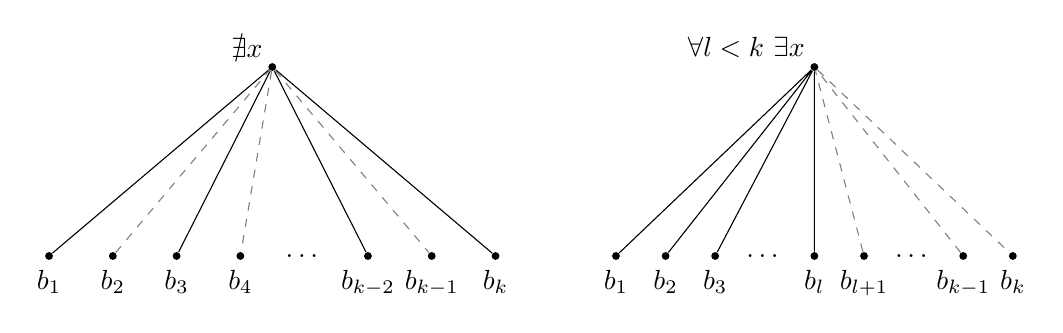
\begin{tikzpicture}[xscale=1.8, yscale=1.2]
      \begin{scope}[xscale=1.8]
        \node [dot, label=below:$b_1$] (1) at (0,0) {};
        \node [dot, label=below:$b_2$] (2) at (0.25,0) {};
        \node [dot, label=below:$b_3$] (3) at (0.5,0) {};
        \node [dot, label=below:$b_4$] (4) at (0.75,0) {};
        \node [dot, label=below:$b_{k-2}$] (5) at (1.25,0) {};
        \node [dot, label=below:$b_{k-1}$] (6) at (1.5,0) {};
        \node [dot, label=below:$b_k$] (7) at (1.75,0) {};
        \node [dot] (8) at (0.875,2) {};
        \node at (1,0) {$\dots$};
        \draw (1) -- (8) -- (3) (5) -- (8) -- (7);
        \draw [dashed, gray] (2) -- (8) -- (4) (8) -- (6);
        \node [above left] at (8) {$\nexists x$};
      \end{scope}

      \begin{scope}[xshift=4cm, xscale=1.4]
        \node [dot, label=below:$b_1$] (1) at (0,0) {};
        \node [dot, label=below:$b_2$] (2) at (0.25,0) {};
        \node [dot, label=below:$b_3$] (3) at (0.5,0) {};
        \node at (0.75,0) {$\dots$};
        \node [dot, label=below:$b_l$] (5) at (1,0) {};
        \node [dot, label=below:$b_{l+1}$] (6) at (1.25,0) {};
        \node at (1.5,0) {$\dots$};
        \node [dot, label=below:$b_{k-1}$] (8) at (1.75,0) {};
        \node [dot, label=below:$b_k$] (9) at (2,0) {};
        \node [dot] (top) at (1,2) {};
        \draw (1) -- (top) -- (2) (3) -- (top) -- (5);
        \draw [dashed, gray] (6) -- (top) (8) -- (top) -- (9);
        \node [above left] at (top) {$\forall l < k \ \exists x$};
      \end{scope}
    \end{tikzpicture}
  \end{center}
  Our idea is to switch from the left picture to the right by replacing $\varphi(x,b_i) \land \neg \varphi(x,b_{i+1})$ by $\neg \varphi(x,b_i) \land \varphi(x,b_{i+1})$ one at a time.
  Along the way, we will switch from an inconsistent set of formulas to a consistent one.

  Specifically, there is $\eta: [k] \to \{0,1\}$ and $l < k$ such that
  \begin{align*}
    \{\varphi^{\eta(i)}(x,b_i) \mid i \neq l, l+1\} \cup \{\varphi(x,b_l, \neg \varphi(x,b_{l+1})\}
  \end{align*}
  is consistent, but
  \begin{align*}
    \{\varphi^{\eta(i)}(x,b_i) \mid i \neq l,l+1\} \cup \{\neg \varphi(x,b_l), \varphi(x,b_{l+1})\}
  \end{align*}
  is inconsistent.

  Let
  \begin{equation*}
  \psi_1(x) = \bigwedge_{i\neq l,l+1} \varphi^{\eta(i)} (x,b_i).
  \end{equation*}
  By indiscernibility of $(b_i)$, $\forall i < j \in \mathbb{Q} \cap [l,l+1]$, we have
  \begin{enumerate}[(a)]
    \item $\psi_1(x) \land \{\varphi(x,b_i), \neg \varphi(x,b_j)\}$ is inconsistent
    \item $\psi_1(x) \land \{\neg\varphi(x,b_i), \varphi(x,b_j)\}$ is consistent.
  \end{enumerate}
  Claim: $\psi(x,y) = \psi_1(x) \land \varphi(x,y)$ has SOP.
  Proof of claim: Take $(b_i') = (b_i \mid i \in \mathbb{Q} \cap [l,l+1])$.
  Then on $b'$, we have $\exists x (\neg \psi(x,b_i) \land \psi(x,b_j)) \leftrightarrow i < j$.
  Indeed, if $i < j$, then
  \begin{align*}
    &\phantom{=}\neg\psi(x,b_i) \land \psi(x,b_j) \\
    &= \neg(\psi_1(x) \land \psi(x,b_i)) \land (\psi_1(x) \land \varphi(x,b_j)) \\
    &= (\neg \psi_1(x) \lor \neg \psi(x,b_i)) \land (\psi_1(x) \land \varphi(x,b_j))
  \end{align*}
  has a solution by b), while if $j \leq i$, it doesn't by a).
\end{proof}

Note we are no longer in the `local' formula setting: this is a statement about theories rather than properties of formulae.

\subsection{Simplicity, forking and dividing}
Throughout, take $T$ countable, complete with infinite models.
\begin{defi}
  Let $k \in \mathbb{N}$. A formula $\varphi(x,y)$ is said to have the $k$-\named{tree property} ($k$-TP) if $(a_\eta)_{\eta \in \omega^{<\omega}}$ such that
  \begin{itemize}
    \item $\forall \eta \in \omega^{<\omega},$ $\{\varphi(x,a_{\eta \wedge i})\}_{i < \omega}$
      is $k$-inconsistent
    \item $\forall \sigma \in \omega^\omega$, $\{\varphi(x,a_{\sigma \mid n})\}_{n < \omega}$ is consistent.
  \end{itemize}
  A theory is $k$-NTP if no formula has $k$-TP.
  A theory is \named{simple} if it is $k$-NTP for all $k \in \mathbb{N}$.
\end{defi}
Informally, the $k$-tree property means that for each node every $k$-family of its children is inconsistent, and every initial segment of the tree is consistent.
\begin{eg}\leavevmode
  \begin{itemize}
    \item Stable theories are simple (exercise)
    \item DLO is not simple (exercise)
    \item The theory of the random graph is simple
    \item The theory of the generic $K_n^r$-free $r$ uniform hypergraph is simple for $n > r > 2$, but not for $n = 3$, $r = 2$.
  \end{itemize}
\end{eg}
\begin{defi}
  Let $k \in \mathbb{N}$, $A$ a small set. A formula $\varphi(x,b)$ is said to $k$-\textbf{divide} over $A$ if there is $(a_i)_{i < \omega}$ such that $\tp(a_i / A) = \tp(b/A)$ for all $i < \omega$, and $\{\varphi(x,a_i)\}_{i<\omega}$ is $k$-inconsistent.

  A formula \textbf{divides} over $A$ if it $k$-divides over $A$ for every $k \in \mathbb{N}$.

  Equivalently, by compactness and the Standard Lemma, $\varphi(x,b)$ $k$-divides over $A$ if there is $A$-indiscernible $(a_i)_{i < \omega}$ starting with $b$ such that $\{\varphi(x,a_i)\}_{i < \omega}$ is $k$-inconsistent.
\end{defi}
\begin{eg}\leavevmode
  \begin{enumerate}
    \item In DLO, the formula $\varphi(x,a) =$ `$x<a$'
      does not divide over $\emptyset$: given any sequence $(b_i)_{i < \omega}$, the type
      \begin{align*}
        \{x < b_i : i < \omega\}
      \end{align*}
      is finitely satisfiable.

      For $a < b$, the formula $\varphi(x,a,b)=$ `$a < x < b$' does divide over $\emptyset$:
      \begin{align*}
        a_1 < b_1 < a_2 < b_2 < \dotsb
      \end{align*}
      $\tp(a_i b_i / \emptyset) = \tp(ab/\emptyset)$, but $\{\varphi(x,a_i,b_i)\}_{i < \omega}$ is 2-inconsistent.
    \item In an arbitrary theory, the formula $\varphi(x,b) = $ `$x = b$' divides over $A$ whenever $b \notin \acl(A)$ (exercise).
    \item In the theory of the random graph, the formula $\varphi(x,a) =$ `$x=a$' divides over $\emptyset$.
      Take an indiscernible sequence starting with $a$, $\{\varphi(x,a_i)\}_{i < \omega}$ will be $2$-inconsistent.

      On the other hand, $\varphi(x,a) =$ `$x \sim a$', `$x \nsim a$', `$x \neq a$' do not divide over $\emptyset$ (the only real way to be inconsistent in the random graph is to try to be equal to two different vertices at once).
      Given any indiscernible sequence $(a_i)_{i < \omega}$ with $a = a_0$, $\{\varphi(x,a_i)\}_{i < \omega}$ is $k$-inconsistent $\forall k \in \mathbb{N}$ by the random graph axioms, for example for any $I \subseteq \omega$ and $|I| = k$,
      \begin{align*}
        \exists x \ x \sim a_i \ \forall i \in I.
      \end{align*}
  \end{enumerate}
\end{eg}
A formula forks over a set if it implies a disjunction of formulas, each of which divide over the set.
This is often useful because it satisfies certain Boolean closure properties.

For simple theories, these two notions coincide.

\lecnum{16}
\begin{prop}[Tent \& Ziegler, 7.24]
  A formula $\varphi(x,y)$ has $k$-TP if and only if $\exists (b_i)_{i < \omega}$ such that $\{\varphi(x,b_i)\}_{i < \omega}$ is consistent but each $\varphi(x,b_i)$ $k$-divides over $\{b_j\}_{j<i}$.
\end{prop}
\begin{cor}
  $T$ is simple  if and only if $\forall \varphi(x,y)$ $\forall k \in \mathbb{N}$, $\nexists (b_i)_{i < \omega}$ such that $\{\varphi(x,b_i)\}_{i<\omega}$ is consistent and $\varphi(x,b_i)$ $k$-divides over $\{b_j\}_{j<i}$.
\end{cor}
\begin{cor}
  If the only formulas that divide are those with finitely many solutions, then $T$ is simple.
\end{cor}
\begin{proof}
  Suppose that $T$ is not simple. By the Corollary,
  there are $\varphi(x,y)$ $k \in \mathbb{N}$, $(b_i)_{i < \omega}$ such that $\{\varphi(x,b_i)\}_{i<\omega}$ is consistent and $\varphi(x,b_i)$ $k$-divides over $\{b_j\}_{j < i}$. This means that for each $i < \omega$, $\exists (b_i^n)_{n < \omega}$ indiscernible over $\{b_j\}_{j < i}$ such that $\{\varphi(x,b_i^n)\}_{n < \omega}$ are $k$-inconsistent and $(b_i^n)_{n<\omega}$ satisfies the same $L(\{b_j\}_{j < i})$ formulas as $b_i$.
  Consider
  \begin{align*}
    \varphi(\mathcal{M},b_0) \supseteq \varphi(\mathcal{M},b_0) \cap \varphi(\mathcal{M},b_1) \supseteq \varphi(\mathcal{M},b_0) \cap \varphi(\mathcal{M},b_1) \cap \varphi(\mathcal{M},b_2) \supseteq \dotsb.
  \end{align*}

  Claim: Containment
  \begin{equation*}
    \bigwedge_{j < i} \varphi(\mathcal{M},b_j) \subsetneq \bigwedge_{j < i} \varphi(\mathcal{M},b_j)
  \end{equation*}
  is proper (so long as the left hand side is non-empty).
  Indeed, let $\psi(y) = \varphi(\mathcal{M},b_j) \wedge \varphi( \mathcal{M}, y)$.
  Then $\psi(b_i^n) \subsetneq \bigwedge_{j < i} \varphi( \mathcal{M} , b_j) $ for some $n < \omega$ for otherwise $\varphi( \mathcal{M} , b_i^n) \supseteq \bigwedge_{j < i} \varphi(\mathcal{M }, b_i)$
  for all $n < \omega$ contradicting the $k$-inconsistency of the $b_i^n$ (if $\bigwedge_{j < i} \varphi( \mathcal{M},b_j) \neq \emptyset$).

  Claim leads to contradiction with consistency of $\{\varphi(x,b_i)\}_{i < \omega}$.
\end{proof}

\begin{eg}\leavevmode
  \begin{enumerate}
    \item In the theory of the random graph, no positive Boolean combination $xRy, \neg x R z$ divides.
      But the theory has QE, so the only formulas which do divide are of the form $\bigwedge \bigvee x=y_i$.
      Each of these only have finitely many solutions, so the random graph is simple.

      Can show that $\varphi(x,\bar{b})$ divides over $A$ if and only if $\varphi(\bar{x},\bar{b}) \rhd x_j = b_i$ for some $x_j\in \bar{x}$ and $b_i \in \bar{b}$.
    \item For $2 \leq k < m$, let $T_{k,m}$ be the theory of the random $K_m^{(k)}$-free $k$-uniform hypergraph.
      (The extension axiom is replaced with: for any $A$ which does not contain a $K_{m-1}^{(k)}$ and any $B$, there is an $x$ etc.)
      This has QE, and is $\aleph_0$-categorical, and is generic in the sense that it contains any $K_m^{(k)}$-free graph.
      \begin{enumerate}[(a)]
        \item $T_{2,3}$ (and more generally, $T_{2,n}$, the Henson graphs) is not simple.
          $\varphi(x,a) = $`$x=a$' divides in the same way as in random graphs.
          On the other hand,
          $\varphi(x,a) = x R a$ does not divide. Indiscernible sequences must be independent sets, so there are no restrictions on types.
          But, the formula $\varphi(x,a,b) = x R a \land x R b$ does divide for $a \neq b$.
          Construct $(a_i,b_i)$ with $a_i R b_j$ iff $i \neq j$ (which is triangle-free, so can be found).
          Now $\{\varphi(x,a_i,b_i)\}_{i<\omega}$ is $2$-inconsistent.
        \item $T_{3,4}$ is simple (Hrushovski)
          Let $\Gamma \models T_{3,4}$ be the countable model, and denote by $R$ the ternary edge relation.
          We look at formulas with infinitely many solutions, and show that none of these divide over the empty set.

          Let $\bar{a}$ be a finite tuple from $\Gamma$, consider $\varphi(x,\bar{a})$ with infinitely many solutions.
          We will show that $\varphi(x,\bar{a})$ does not $k$-divide over the empty set for any $k$.

          Let $(\bar{a_i})_{i < \omega}$ be an indiscernible with $\bar{a_0} = \bar{a}$.
          Need to show that $\{\varphi(x,\bar{a_i}\}_{i < \omega}$ is consistent.

          Fix $N \in \mathbb{N}$. For each $i \leq N$, let $A_i$ be the set of elements of $\bar{a_i}$.
          Construct a $3$-uniform hypergraph $\Delta$ as follows:
          the vertex set of $\Delta$ is $\bigcup_{i < N} A_i \cup \{c\}$ for some new point $c$ (not in $\Gamma$).
          The edges on triples of $\Delta$ are as induced by $\Gamma$:
          \begin{itemize}
            \item if $\bar{b} \subseteq \Gamma$, then $\bar{b}$ is an edge in $\Delta$ if and only if it is an edge in $\Gamma$, i.e.\ $R(\bar{b})$ holds.
            \item if $c \in \bar{b}$, $\bar{b}$ is an edge in $\Delta$ if and only if $\bar{b}\ \{c\} \subseteq A_i$ for some $i$ and $\varphi(x,\bar{a}) \vdash R(x,\bar{b}\setminus \{c\})$

              (For instance, if $\varphi(x,\bar{a_i}))$ might say $R(x a_i^1 a_i^2)$ but $\neg R(x a_i^2  a_i^3)$.
              Then $\bar{b} = c a_i^1 a_i^2$ will be an edge in $\Delta$, while $c a_i^2 a_i^3$ will not).
          \end{itemize}
          Claim: $\Delta$ is $K_4^{(3)}$-free.
          Once we have this claim, we have that $\Delta$ embeds into $\Gamma$, so there is a point in $\Gamma$ that behaves like $c$, so $\{\varphi(x,\bar{a_i})\}_{i \leq N}$ is consistent.

          Proof of claim. Suppose we have a $K_4^{(3)}$. Then $c$ is one of the vertices.
          Aim to say that $B \setminus \{c\} \subseteq A_i$ for some $i$.
      \end{enumerate}
  \end{enumerate}
\end{eg}
\printindex
\end{document}
